\documentclass{article}
\usepackage{graphicx} % Required for inserting images
\usepackage[backend=biber, style=numeric]{biblatex}
\addbibresource{references.bib}
\usepackage{amsmath}
\usepackage{amssymb}
\usepackage[margin=1in]{geometry}
\usepackage{booktabs}
\usepackage{array}
\usepackage{multirow}
\usepackage{float}


\usepackage{listings}
\usepackage{xcolor}

\lstdefinestyle{pythonstyle}{
    language=Python,
    basicstyle=\ttfamily\small,
    keywordstyle=\color{blue},
    stringstyle=\color{green!50!black},
    commentstyle=\color{gray},
    numbers=left,
    numberstyle=\tiny\color{gray},
    frame=single,
    breaklines=true,
    showstringspaces=false,
    tabsize=4
}



\title{Performance of different machine learning methods on predicting the result of a football match}
\author{Michal Grega \\
  \texttt{migre@itu.dk} \\
  \texttt{IT university of Copenhagen}}
\date{August 2026}

\begin{document}

\maketitle
\section*{Abstract}
Predictions for football matches have always been a notoriously difficult task because of the three way outcome of a match, also called 1X2 betting. What is especially difficult is to determine the cases where neither team has the edge, therefore predicting a draw. In this paper, different machine learning methods are applied to tackle this task and to see whether some are better suited for this problem than others. The dataset used for predictions consists of historical records, specifically the last 12 seasons of the English Premier League (2014-2026). The dataset was enriched with additional features, such as rolling averages of the features, points per game, team elo ranking and expected goals (xG). The models were evaluated on their log loss and Brier score. The models used could be divided into discriminative and generative. The discriminative models include a feed-forward neural network, ensemble methods as random forest and gradient boosting, multinomial Logistic regression and Support vector machines. The generative models include different algorithmic extensions of a Poisson regression. The main purpose of this paper is to maximize the predictive performance of the generative Poisson model and compare it to other common methods in the industry, such as the ensembles, as a reference point. All the models were evaluated on their performance of the 1X2 prediction task and compared to the bookmakers' odds as well as a baseline model that predicts the most likely outcome based on the historical distribution of the target variable. The results show that all the models fall short of the bookmakers' odds, however, the best performing model was the bivariate Poisson regression with covariates, which was just marginally underpreforming the market. This was the result of finding ways via algorithmic improvements as well as reducing the features space. Despite the other models trailing by a larger margin, they all very comfortably outperform the baseline model, which is a clear indication that the methods used in this paper are able to capture the signal in the data and learn patterns that are relevant for the prediction task. The results of this paper can be used as a reference point for future research in this area, as well as a benchmark for other models that are used in the industry.

 
\section{Introduction}
Gambling on sports has been long part of the world but only fairly recently has this field been so mapped out and researched. Statistical models have allowed the odds providers to expand to a much larger scale and with well-calibrated odds bringing unprecedented precision. Since statistical/machine learning models are at the very core of the source of profit that these odds providers gain, there are not any publicly available fully  documented data about this topic. The objective of this paper is to search for which methods perform well in predicting sports outcomes and could potentially be used on an industrial scale. The exact objective of prediction is the threeway betting in football, also known as 1X2 betting. While there are many options to predict in today's game that is full of match statistics and odds providers offer multitude of different things to bet on, such as amount of shots or corners taken in the game, the threeway betting is the most popular as well as most obscure and interesting to research. Majority of statistics in a football match can go two ways - either there will be more or less of some observed statistic, such as asking "Will there be more or less than 8 shots on goal in this match?". This is a trivial case where the model tries to find the most precise value as a splitting point. However, the 1X2 bet is substantially more difficult, not only because there is simply one more option to consider, but especially because the X (draw) is very troublesome to predict. It does not occur that often and the factors that would typically indicate a win of either 2 teams are much weaker in favouring a draw, in other words, a draw is rarely ever considered the most probable outcome of a match. However, the task at hand is not to make a cardinal prediction but rather a probabilistic output for all three possibilities. 
\\
This paper goes through the whole process of how such task could be carried out - from the data extraction to feature engineering followed by classification of the different statistical and machine learning models and evaluation of the results and conclusion circling back to the objective of this paper.


\section{Methodology}
To approach a problem, we firstly need to define it in rather strict terms. What we aim for in this paper is to predict the outcome of a football match. Meaning, we predict whether a football match is either going to be won by one or the other team or the result will be a draw. This kind of format is also called 1X2 in the betting industry. The 1 stands for home team win, X for a draw and 2 for the away team win. For this task, different kind of machine learning algorithms will be applied and evaluated based on their metrics. For training the ML models, it is of great importance to choose a dataset rich in information and possible signal for the algorithms to learn and distinguish important patterns that may give the edge towards a correct prediction. The methodology of this paper could be defined in these steps:

\begin{itemize}
    \item \textbf{Data exploration} Finding a dataset that is rich in information and contains the relevant features for the prediction task. Following that, the dataset is explored to find any patterns or distribution shifts that may occur over time. This includes inspecting the distribution of the target variable, as well as the distribution or other observations of the features selected for training.
    \item \textbf{Feature engineering} Creating new features that may be relevant for the prediction task. This includes creating rolling averages of the features, as well as creating new features such as points per game, team elo ranking and expected goals (xG). This goes hand in hand with training the models and evaluating their performance, e.g some features do not serve any purpose and are rather creating noise than signal. Therefore this also includes feature selection practices, such as permutation importance and gini impurity feature importance. This is also accompanied by scaling the data upwards which is another technique used in attempt to boost the performance of models. On top of exploring the feature space, it is also beneficial to simply add more matches to the training data. In this paper the data however comes from a single league, meaning that adding data represents adding older seasons within the same league. This is a trade-off between adding more data and the distribution shift that occurs over time, as the game of football evolves and changes over time. A similar issue would be raised by adding data from other leagues, as the style of play is different and therefore the distribution of features would be different as well.
    \item \textbf{Machine learning and statistical models} Model selection happens in the feature engineering phase already, where there is sort of a baseline created and everything that follows aims at one goal; to improve the performance of the models. The models are built and trained on the dataset, with the goal of maximizing their predictive performance. This includes hyperparameter tuning, as well as inference of different architectures, especially going particularly deep in the generative models.
    \item \textbf{Data splitting} Different ways of splitting the data are explored, such as training a single season and testing on the next one, training and testing within a single season or training multiple seasons and testing on the next one. There are certain limitations due to time series nature of the data. For some models it is also necessary to leave out a portion of data for validation purposes to avoid overfitting.
    \item \textbf{Evaluation} As well as other points in the methodology, evaluation is an ongoing process that is done throughout the majority of the project. The baseline models are evaluated on the simple and intuitive accuracy metric. In the case of 1X2 betting, accuracy is treated as an \texttt{argmax} function. The model outputs three probabilities for a match and whichever is the highest, that is treated as the models final prediction. That is also why the recall of draws is very low because this method only ever chooses the highest probability outcome and the draw is almost never that. Despite delivering the incomplete message, it has been proven in the results that accuracy is highly correlated with the more insightful measurements of performance on probabilistic outputs - log loss and Brier score. Therefore, it is deemed a sufficient metric for the baseline versions of models that are explored in this paper. However, as the models progressed along the feature space, log loss and Brier score were the primary target for optimization. These two metrics are targeted for evaluation of probabilistic outputs that take into consideration the confidence of the model. If the model predicts an event with 51\% probability and another does so with 90\% probability, it is a significant difference in confidence. If such outcome happens to be true, these metrics will punish the 51\% prediction much more than the 90\% one because of how uncertain the first prediction was. However, if the outcome happens to be different, the model that was very certain and eventually wrong will get severely punished instead. Accuracy is blind to the confidence factor in predictions, which is the most important factor in the betting industry.
    
\end{itemize}

\section{Feature space}
\subsection{Dataset}
The dataset is curated from https://www.football-data.co.uk/, which provides the raw match statistics that most of the engineered features are built from. Not every raw feature proved useful for the 1X2 prediction task, so several were added on top: rolling averages of the existing statistics (and the home/away difference between them), team Elo ratings, points per game, and expected goals, summarized in Table~\ref{tab:feature_categories}. Shot accuracy, absent from the raw data, was computed directly as goals scored divided by total shots. As found during EDA, the rolling features are grouped by venue as well as by team, since a team's home and away form can differ meaningfully - the exact construction of these rolling averages is detailed in the Moving average subsection.





\subsection{Exploratory data analysis}
The dataset available contains the last 12 seasons of the English Premier League (2014-2026), each season having 380 matches, that would add up to 4560 matches in total (this is disregarding the dropping of first round matches each season that is baked into the moving average logic). 
Distribution shift occurs in many aspects of the game when looking at football over a decade ago. Victoria Kereki in her paper about FC Barcelona's tactical Evolution (2004–2021) \cite{Distribution_shift} talks about how clearly the game has changed when doing a clustering analysis on their passes throughout the years. In the span of 12 years of the English Premier League (EPL), there have also been noticeable changes in game patterns.  

\begin{figure}[H]
    \centering
    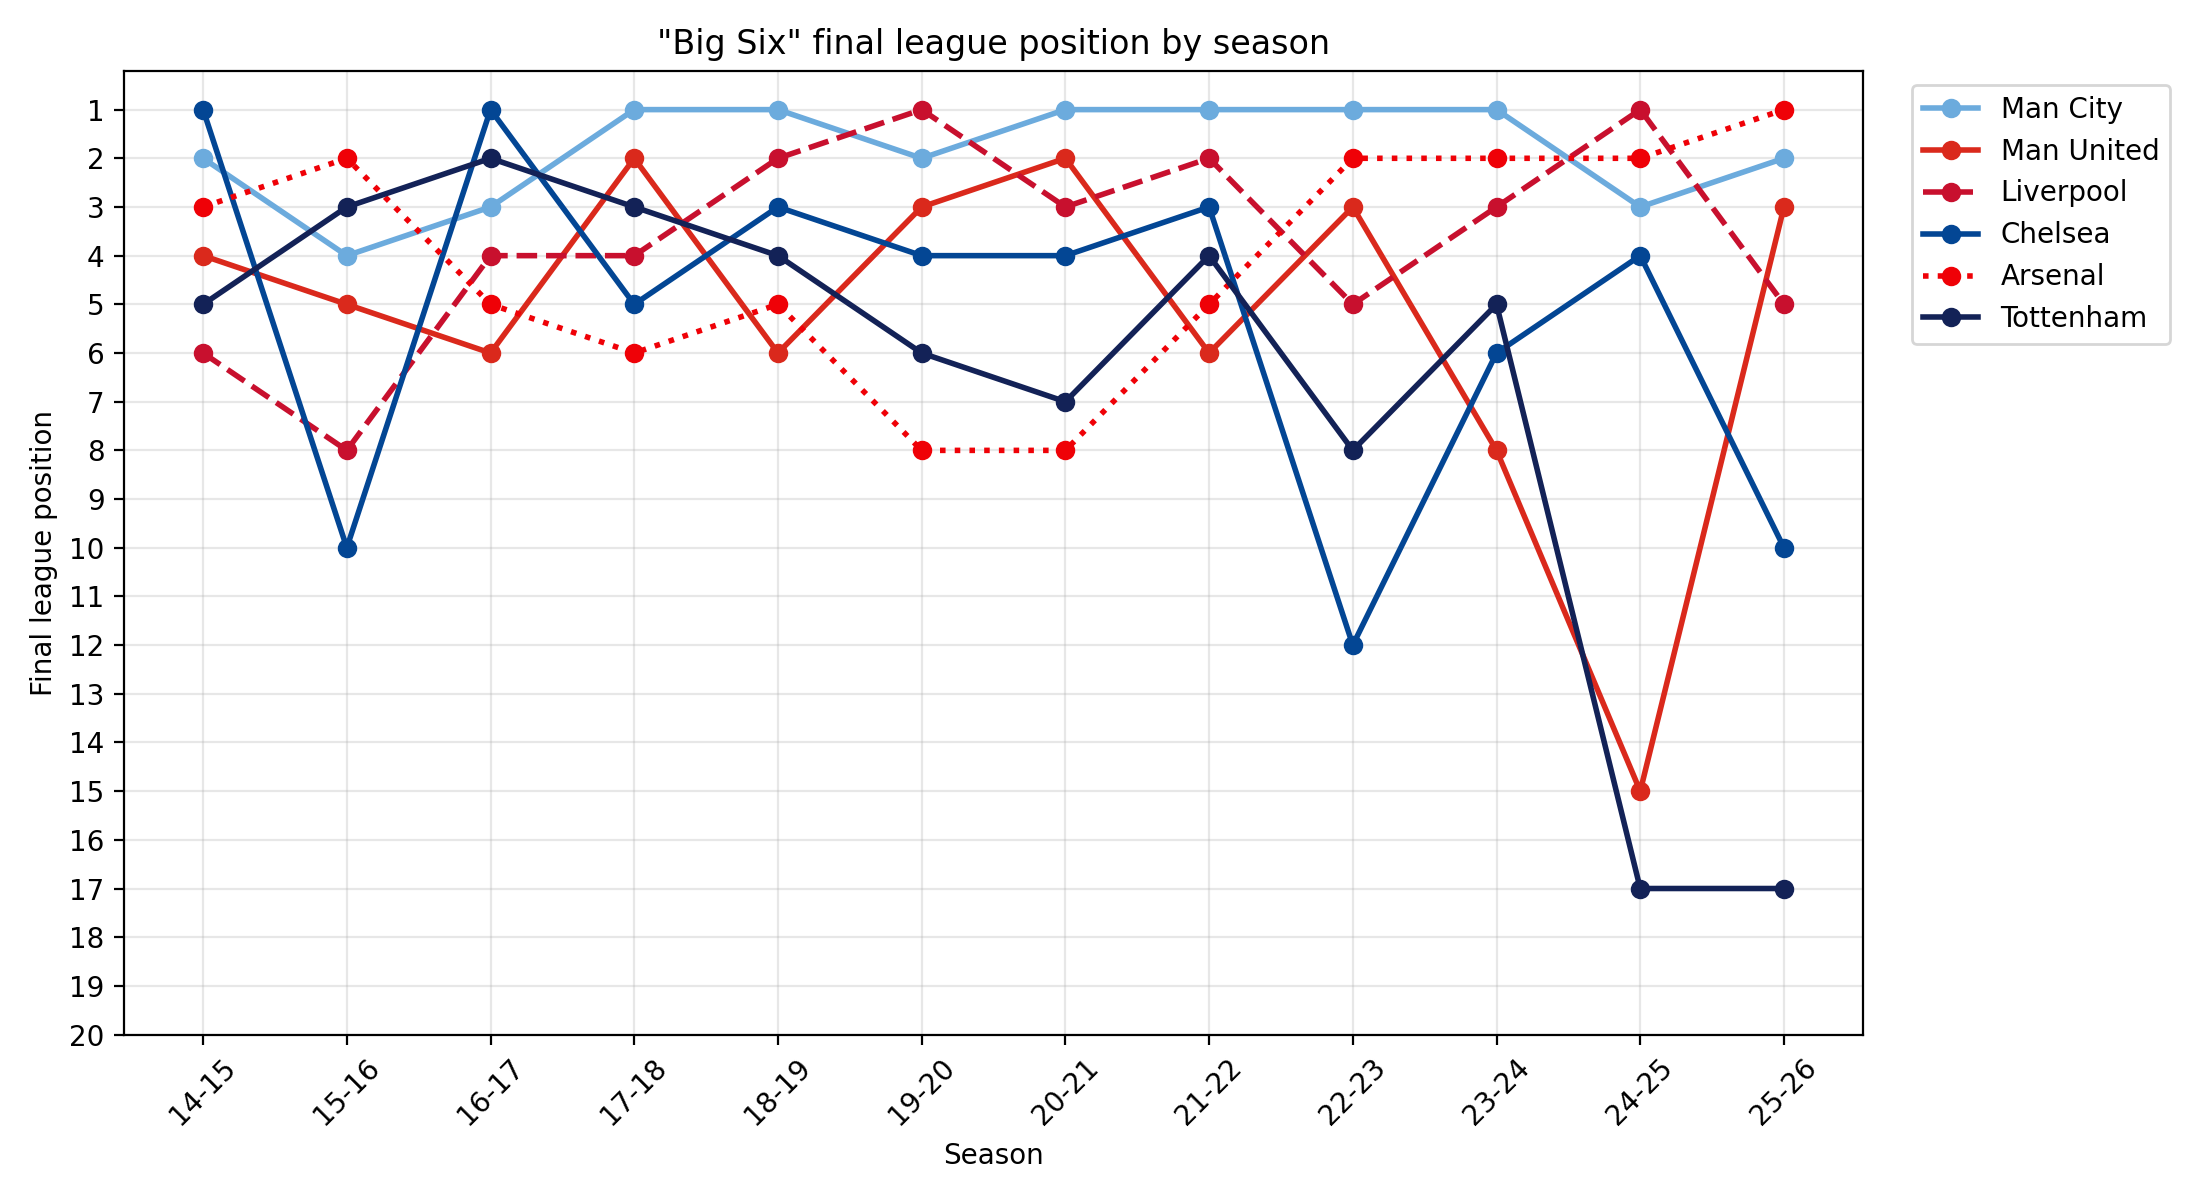
\includegraphics[width=0.7\linewidth]{images/eda_bigsix.png}
    \caption{The "Big six" }
    \label{fig:bigsix}
\end{figure}

Naturally, teams develop over time, whether into a good or bad direction. Figure \ref{fig:bigsix} shows final standings in all 12 seasons of the so called "Big six" - group of the most successful teams in the EPL. There is an apparent trend in recent years that shows a large variance in the final standings between most of these teams. This clearly indicates unpredictability. Moreover, the winner of 2015-16 EPL, Leicester, has in the 2025-26 season been relegated to League one - the \textbf{third} best league in England, further proving the volatility and competitiveness of the league. The reason for such a variety of final standings in the league could be associated with a number of things, such as changes in team tactics, coach, players or clubs' management and financial status. Another evidence of a distribution shift can be seen on the figure \ref{fig:home_adv} below.

\begin{figure}[H]
    \centering
    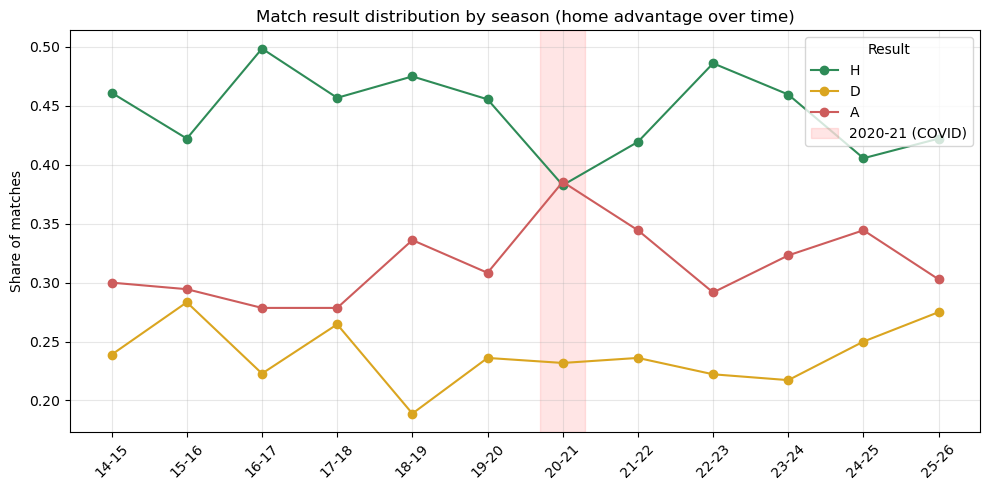
\includegraphics[width=0.7\linewidth]{images/eda_home_adv.png}
    \caption{The home advantage distribution }
    \label{fig:home_adv}
\end{figure}

Home advantage has been very evident throughout all the seasons except one, when there were empty stadiums during the games due to Covid. This factor can negatively impact the predictions of a model, that naturally learns patterns about home advantage in prior seasons. The figure also shows the distribution of the target feature itself - the full time result of a game. Draws have always been the least likely outcome, even though often almost on equal with the away team wins.
\\
Looking at the shots on target in figure \ref{fig:sot} can also reveal some information about the trend over the last 12 years.

\begin{figure}[H]
    \centering
    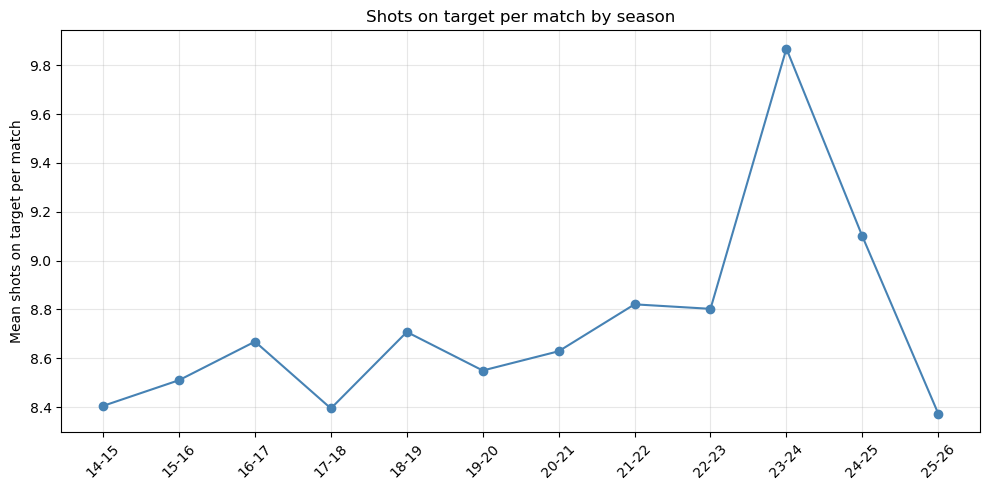
\includegraphics[width=0.7\linewidth]{images/eda_sot.png}
    \caption{The shots on target distribution }
    \label{fig:sot}
\end{figure}

More shots on target results in more goals as well and in the EPL, they have been quite consistent throughout the years, except from the 2023-24 season, that is effectively an outlier, as the shots on target dropped rapidly in the following seasons again. 
\\
When plotting the overall count of goals per match in all the seasons together, an interesting pattern occurs. 

\begin{figure}[H]
    \centering
    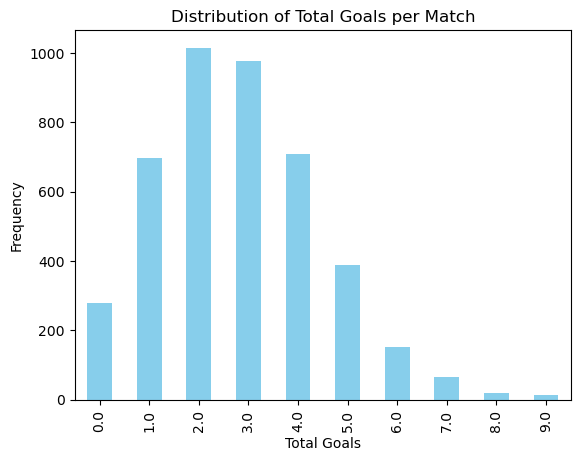
\includegraphics[width=0.7\linewidth]{images/goals_distribution.png}
    \caption{Distribution of total goals per match }
    \label{fig:goals_dist}
\end{figure}
The distribution of goals per match in figure \ref{fig:goals_dist} happens to follow the well-known Poisson distribution and it is tested by the 
$\chi^2$ goodness-of-fit test on the total number of goals
scored per match (home plus away), pooled across all 12 seasons in the dataset ($n = 4315$ matches).

The rate parameter $\hat{\lambda}$ was estimated via maximum likelihood as
the sample mean:
\[
\hat{\lambda} = \bar{x} = \frac{1}{n}\sum_{i=1}^{n} x_i = 2.8019
\]
with sample variance $s^2 = 2.7394$, close to $\hat{\lambda}$ as expected
under the Poisson equidispersion property ($\mathrm{Var}(X) = \mathbb{E}[X]$).

Under the null hypothesis $H_0$: total goals per match $\sim \mathrm{Poisson}(\hat{\lambda})$,
the expected count in bin $k$ is
\[
E_k = n \cdot P(X = k) = n \cdot \frac{\hat{\lambda}^k e^{-\hat{\lambda}}}{k!}
\]
for $k = 0, 1, \dots, 6$, with the tail bin ($k \geq 7$) pooled to keep
expected counts sufficiently large:
\[
E_{7+} = n \left(1 - \sum_{k=0}^{6} P(X=k)\right)
\]

Table~\ref{tab:poisson_gof} reports the observed ($O_k$) and expected
($E_k$) counts per bin.

\begin{table}[H]
\centering
\caption{Observed vs.\ expected total-goals-per-match counts under $\mathrm{Poisson}(\hat{\lambda}=2.802)$}
\label{tab:poisson_gof}
\begin{tabular}{lcc}
\toprule
\textbf{Goals} & \textbf{Observed} $O_k$ & \textbf{Expected} $E_k$ \\
\midrule
0    & 279  & 261.91 \\
1    & 696  & 733.83 \\
2    & 1015 & 1028.04 \\
3    & 975  & 960.14 \\
4    & 709  & 672.55 \\
5    & 389  & 376.87 \\
6    & 153  & 175.99 \\
7+   & 99   & 105.66 \\
\bottomrule
\end{tabular}
\end{table}

The Pearson $\chi^2$ test statistic is
\[
\chi^2 = \sum_{k} \frac{(O_k - E_k)^2}{E_k} = 9.2502
\]
with $\mathrm{dof} = (\text{bins} - 1) - (\text{estimated parameters}) = 8 - 1 - 1 = 6$
(one degree of freedom is lost for estimating $\hat{\lambda}$ from the data).
This yields
\[
p = 0.1600
\]

Since $p > 0.05$, the null hypothesis is not rejected: the observed
distribution of total goals per match does not deviate significantly from a Poisson distribution. This represents the key underlying assumption for the generative models in this paper.








\subsection{Feature importance}
To avoid any ambiguity in the choice of features that would pass through feature selection, a simple random forest model was run on the dataset, using the features that have the possibility to carry the information that is readily available before the match, not during it, therefore rendering the \texttt{Half-time result} and \texttt{Half-time home and away goals} features unusable. After the inference, the \texttt{feature\_importances\_} method from \texttt{sklearn} determined the features' importance based on impurity of the leafs in the decision trees shown in \ref{tab:feature_importance}.
\begin{table}[H]
\centering
\begin{tabular}{@{} l c @{}}
\toprule
\textbf{Feature} & \textbf{Importance} \\
\midrule
AST (away shots on target) & 0.2784 \\
HST (home shots on target) & 0.2612 \\
AS (away shots)             & 0.1213 \\
HS (home shots)              & 0.0930 \\
AF (away fouls)              & 0.0444 \\
AC (away corners)            & 0.0418 \\
AY (away yellows)            & 0.0390 \\
HF (home fouls)              & 0.0388 \\
HC (home corners)            & 0.0376 \\
HY (home yellows)            & 0.0313 \\
HR (home reds)               & 0.0104 \\
AR (away reds)               & 0.0027 \\
\bottomrule
\end{tabular}
\caption{Feature importance ranking}
\label{tab:feature_importance}
\end{table}
The feature importance function revealed the features that this random forest model was making it's decisions based on. That is one way to address the issue of feature selection. On this basis, the shot features, especially the ones on target, were dominant. On the other hand, red card features rank very poorly, in the 0.01-0.002 territory. The final decision was to cut out the red card features as they were by far the smallest, negligible contributor to the model.

The current state of the feature space offers a baseline selection of predictors for the match outcome. However, despite these features representing the essential statistics of a football game, the accuracy of the model could be improved with more advanced predictors in the dataset. That is why it is necessary to look further and take the feature selection to another level. 


\subsection{Points per game}
Another way of capturing the strength of a team are their respective points per game. This directly encapsulates team strength not just in terms of their shots or fouls they make, but the points they gain over the course of the season. This is naturally a floating point number between 0 to 3 and is updated after each match a team has played.


\subsection{Team elo ranking}
One of the extra features that do not occur in the original dataset is called Elo. Elo ranking was first introduced for determining the relative skill level of chess players \cite{ELO}. In the case of football statistics, it is an adaptation of the original formula, with a twist of considering the magnitude of win, namely the goal difference, rather than a simple win/loss scenario that occurs in chess. 
\\
The expected outcome for the home team is given by:
\begin{equation}
E_H = \frac{1}{1 + 10^{-\left(R_H - R_A\right)/400}}
\end{equation}

\begin{description}
    \item[$E_H$] Expected score (probability of winning) for the home team, $E_H \in [0,1]$.
    \item[$R_H$] Current Elo rating of the home team (values between 1500-2090).
    \item[$R_A$] Current Elo rating of the away team (same values as for the home elo).
\end{description}

The corresponding rating update after the match is played is:
\begin{equation}
R_H' = R_H + K \cdot G \cdot \left( S_H - E_H \right)
\end{equation}

\begin{description}
    \item[$R_H'$] Updated Elo rating for the home team after the match.
    \item[$K$] Development constant controlling the maximum possible rating adjustment per match.
    \item[$G$] Goal-difference multiplier, scaling the rating change according to the margin of victory (commonly used in football Elo variants, e.g., the World Football Elo Ratings system).
    \item[$S_H$] Actual match outcome for the home team: $S_H = 1$ for a win, $S_H = 0.5$ for a draw, $S_H = 0$ for a loss.
    \item[$E_H$] Expected outcome for the home team, as defined above.
\end{description}

A common specification for the goal-difference multiplier $G$, used by the World Football Elo Ratings \cite{Elo}, is:
\begin{equation}
G =
\begin{cases}
1 & \text{if goal difference} = 0 \text{ or } 1 \\
1.5 & \text{if goal difference} = 2 \\
\dfrac{11 + \left| \text{goal difference} \right|}{8} & \text{if goal difference} \geq 3
\end{cases}
\end{equation}

Since Elo rating is already capturing a lot of the information about wins and losses and the goals scored while being relative to each team's strength, it is considered to be the cornerstone of the feature dataset. 
\\
Elo ratings are obtained via the http://www.clubelo.com API. Filtering based on team's name, every single match in the dataset contains the current team's elo rating at a time. This elo rating is being updated consequently following the formula explained earlier in this section so that it encapsulates the long term strength of a team but carries information about the recent form as well. 



\subsection{Moving average}
First and foremost, when predicting a match result before the data is available, it is necessary to have some data to feed the model beforehand. This can be provided by the previous matches of both teams. Therefore, this problem is handled by computing the moving averages of the features used in the dataset. The size of the window chosen was based on running a sweep over a range of configurations. Instead of a plain rolling average, Exponentially weighted moving average (EWMA) was used. 
\begin{equation}
\text{EWMA}(t) = \alpha \cdot x(t) + (1 - \alpha) \cdot \text{EWMA}(t-1)
\end{equation}

\begin{itemize}
    \item $x(t)$ is the current data point, floating point number representing any value from the feature space.
    \item $\alpha$ is the smoothing factor, value between 0 and 1. The higher the value the more weight added to recent data. The exact value used here is 0.133 which is explained later.
    \item $\text{EWMA}(t-1)$ is the previous EWMA value.
\end{itemize}

Intuitively, the recent form for sports such as football means last few matches, however, with the feature engineering loop through the moving average window, it has been proven that the convergence of model's log loss was reached at number 14. This is a number that represents over half of a single season, when it comes to the features that are grouped by venue for a team. To be precise, since each team plays 38 matches in total, split equally in home and away venues, the moving average window spans across 14/19 = ~74\% of seasonal matches, for the venue specific features. This might seem like a lot, but that is exactly why the EMWA is such a good fit. Ability to capture smoothed signal from the data while prioritizing the most recent matches is what separates this method from a vanilla rolling average. For reference, the smoothing factor is using the standard \texttt{Pandas} formula that scales the smoothing factor according to the span size; $\alpha$ = 2 / (span + 1).
Half-life (time for a weight to decay to 50\%): solve $(1-\alpha)^h = 0.5$ for $h$.
With $\alpha = 2/15$, $1-\alpha = 13/15 \approx 0.8667$:

\begin{equation}
\alpha = \frac{2}{\text{span}+1} = \frac{2}{14+1} = \frac{2}{15} \approx 0.1333
\end{equation}

\begin{equation}
w_k = \alpha (1-\alpha)^k
\end{equation}

\begin{equation}
h = \frac{\ln(0.5)}{\ln(1-\alpha)} = \frac{\ln(0.5)}{\ln\left(\dfrac{13}{15}\right)} \approx \frac{-0.6931}{-0.1431} \approx 4.84 \text{ matches}
\end{equation}

Contribution of the match at the span boundary (14 matches back, relative to the most recent match's weight): the weight of an observation $k$ lags back is $w_k = \alpha(1-\alpha)^k$, so the ratio to the most recent ($k=0$) is just $(1-\alpha)^k$.

\begin{equation}
\frac{w_{14}}{w_0} = (1-\alpha)^{14} = \left(\frac{13}{15}\right)^{14} \approx 0.1349 \;\; (13.49\%)
\end{equation}

For $k=14$: $(13/15)^{14} \approx 0.1349$ → the match 14 games back contributes ~13.5\% as much as the most recent one.
\\
To clarify  the reason for EMWA; simple rolling average over last few matches does not capture the signal of features as realistically as factoring in the recency with a decay the further the match has been played in the past. While in a naive implementation of the moving average, all the matches would have a same weight, EMWA stresses the importance of most recent match much more than the last one in the spanning window - in this case the last match (14th) is contributing only a 13.5\% of the most recent one. This also allows for increasing the moving window size perhaps much beyond intuition.



\subsection{Expected goals (xG)}
Another feature that is a great contributor to the explanation of the variance in data is the xG statistic. An expected goals model tries to estimate the probability of any given shot being converted to a goal based on various different factors describing the shot. These probabilities can then be added up per team and yield a “result-agnostic” description of the teams' performance \cite{xG}. The xG feature alone is estimated by a supervised machine learning model that outputs a probabilistic number between 0 and 1. Whichever discriminative method used, features such as shot location, speed of player taking the shot, defenders in the line of the shot or goalkeepers position are pivotal in the xG estimation.
\\
The xG values were obtained from Understat.com, a third-party analytics provider. It is important to note that Understat's exact xG model is proprietary and not published in peer-reviewed literature; the values used here should be treated as an externally-validated but non-transparent measure of chance quality.

\subsection{Selecting features}
The base feature space has grown massively and there might be a need for some structural cleansing of the dataset e.g feature selection. Knowledge about which features carry the strongest signal for predictions can also be beneficial later. Upon conducting the same feature importance function from \texttt{sklearn} again as before, the results are much different. The previous feature engineering subsection introduced a number of features that overtook the lead in the ranking of important features that the random forest model uses to base its decisions on. In table \ref{tab:feature_importance_v2} with the top 15 important features in gini impurity, it is clear that the \texttt{Elo\_difference} feature dominates and carries the most signal. It is also one of the most complex features in the dataset as it is using the relative strength of teams and the level of dominance in their games.
\begin{table}[H]
\centering
\begin{tabular}{@{} c l c @{}}
\toprule
\textbf{Rank} & \textbf{Feature} & \textbf{Importance} \\
\midrule
1  & Elo\_Difference                              & 0.0810 \\
2  & PPG\_Difference                               & 0.0436 \\
3  & Home\_ShotOnTargetDifference\_Rolling        & 0.0352 \\
4  & Home\_ShotOnTargetDifference\_RollingTeam    & 0.0252 \\
5  & Home\_Elo                                     & 0.0220 \\
6  & Home\_ShotDifference\_Rolling                & 0.0217 \\
7  & Home\_deep\_Rolling                          & 0.0215 \\
8  & Home\_ShotsOnTarget\_Rolling                 & 0.0213 \\
9  & Home\_Shots\_Rolling                         & 0.0203 \\
10 & Away\_ShotOnTargetDifference\_RollingTeam    & 0.0196 \\
11 & Away\_Elo                                     & 0.0194 \\
12 & Away\_xG\_RollingTeam                        & 0.0194 \\
13 & Away\_ShotDifference\_RollingTeam            & 0.0193 \\
14 & Home\_xG\_Rolling                           & 0.0191 \\
15 & Home\_GoalDifference\_Rolling                & 0.0177 \\
\bottomrule
\end{tabular}
\caption{RF Feature importance ranking after increasing the feature space}
\label{tab:feature_importance_v2}
\end{table}

Another method for determining the features that carry the most signal is the Permutation feature importance, also an implementation from \texttt{sklearn}. This time the train/test set is split into all seasons before 2025-26 as training portion and this last season as a held-out split. Features in the held-out set (test set) are randomly shuffled one by one, model is tested and the degradation of the log-loss of the model is then reported for each feature. The higher the degradation of log loss means the particular feature that was shuffled carried more significant signal. The values in table \ref{tab:permutation_importance} show a marginal difference of performance improvement that the feature provide, shots on target being the highest ranked. Despite the subtle differences in rankings, there is a large overlap in the findings from both gini impurity based as well as permutation feature importance experiments.


\begin{table}[H]
\centering
\begin{tabular}{@{} c l c @{}}
\toprule
\textbf{Rank} & \textbf{Feature} & \textbf{Mean $\Delta$ log loss} \\
\midrule
1  & Home\_ShotOnTargetDifference\_Rolling     & +0.0016 \\
2  & Home\_ShotOnTargetDifference\_RollingTeam & +0.0013 \\
3  & PPG\_Difference                             & +0.0013 \\
4  & Home\_Shots\_Rolling                       & +0.0012 \\
5  & Elo\_Difference                             & +0.0010 \\
6  & Home\_ShotDifference\_RollingTeam          & +0.0010 \\
7  & Home\_ShotsOnTarget\_Rolling                & +0.0009 \\
8  & Home\_xGA\_Rolling                         & +0.0008 \\
9  & Home\_ShotDifference\_Rolling               & +0.0008 \\
10 & Home\_deep\_Rolling                         & +0.0008 \\
11 & Home\_GoalDifference\_RollingTeam           & +0.0005 \\
12 & Away\_PPG                                    & +0.0004 \\
13 & Home\_GoalDifference\_Rolling                & +0.0004 \\
14 & Home\_xGA\_RollingTeam                      & +0.0004 \\
15 & Away\_ShotAccuracy\_Rolling                  & +0.0003 \\
\bottomrule
\end{tabular}
\caption{Permutation feature importance ranked by mean $\Delta$ log loss}
\label{tab:permutation_importance}
\end{table}



The feature importance tests are followed by Pearson correlation tests for multicollinearity inside the feature space in figure \ref{fig:feature_correlation}. These are again conducted on the top selection of features only. 








\begin{figure}[H]
    \centering
    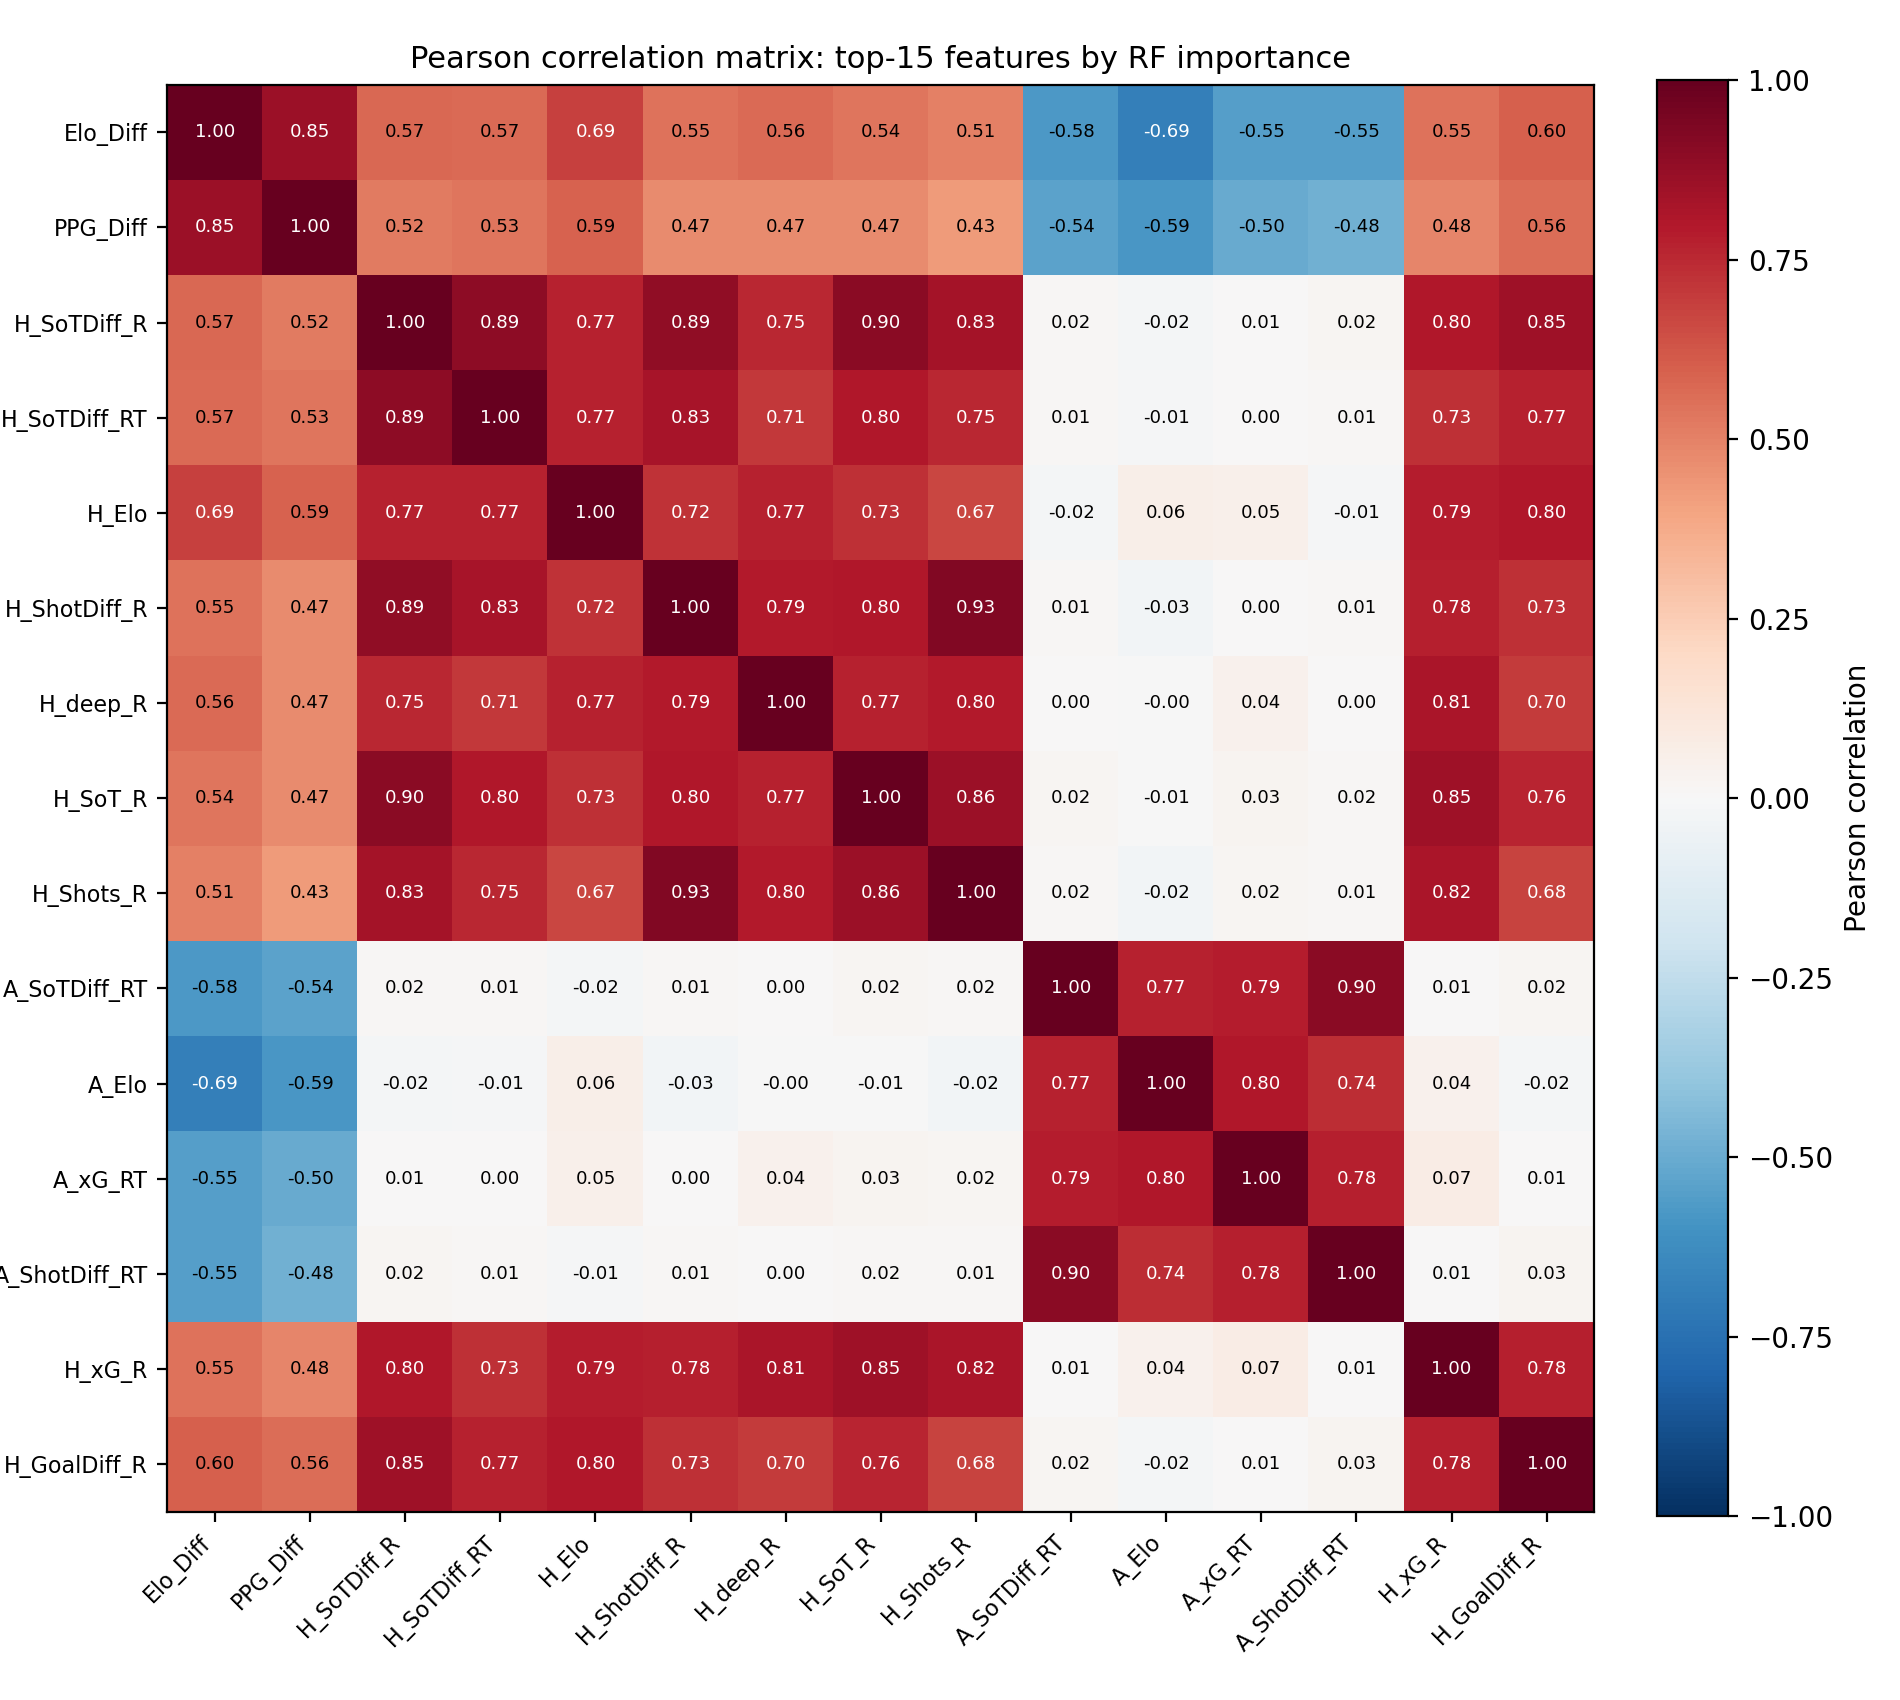
\includegraphics[width=0.95\linewidth]{images/feature_correlation_matrix.png}
    \caption{Pearson correlation matrix of the 15 features in Table~\ref{tab:feature_importance_v2}.}
    \label{fig:feature_correlation}
\end{figure}

The matrix reveals substantial multicollinearity within the home-side rolling shot/xG/goal-difference features (many pairwise correlations above 0.8, e.g.\ \texttt{Home\_ShotDifference\_Rolling} and \texttt{Home\_Shots\_Rolling} at $r=0.93$), as expected since they are all rolling summaries of closely related underlying match events. The away-side features form a similarly tight, largely separate cluster, and are close to uncorrelated with the home-side cluster ($|r|$ mostly below 0.05), while \texttt{Elo\_Difference} and \texttt{PPG\_Difference} are strongly correlated with each other ($r=0.85$) and negatively correlated with the away-side cluster ($r\approx-0.5$ to $-0.7$), consistent with them being difference features that mix information from both teams.
\\
The multicollinearity trend follows down the line of all the 96 features that are found in the dataset. However, as the objective of this paper is to maximise the performance of models on the 1X2 prediction of football matches, as long as the features provide signal that strenghtens the predictive power then the multicollinearity is not regarded as a major issue. First reason for this is that interpreting the individual coefficients is not of the highest importance and secondly, due to the low amount of data entries, it is not computationally expensive to include more features.

Table~\ref{tab:feature_summary_stats} reports summary statistics for these same 15 features.

\begin{table}[H]
\centering
\resizebox{\linewidth}{!}{%
\begin{tabular}{lccccccc}
\toprule
\textbf{Feature} & \textbf{Mean} & \textbf{Std} & \textbf{Min} & \textbf{25\%} & \textbf{50\%} & \textbf{75\%} & \textbf{Max} \\
\midrule
Elo\_Difference                          & 0.102    & 162.360 & -482.202 & -107.050 & -2.701 & 107.409 & 511.554 \\
PPG\_Difference                           & -0.013   & 0.767   & -2.400   & -0.531   & 0.000  & 0.500   & 2.667   \\
Home\_ShotOnTargetDifference\_Rolling     & 0.801    & 1.940   & -7.139   & -0.534   & 0.498  & 1.938   & 6.713   \\
Home\_ShotOnTargetDifference\_RollingTeam & -0.034   & 1.864   & -5.679   & -1.355   & -0.277 & 1.135   & 6.136   \\
Home\_Elo                                 & 1750.634 & 118.237 & 1499.452 & 1658.755 & 1733.023 & 1832.008 & 2088.262 \\
Home\_ShotDifference\_Rolling             & 2.604    & 4.777   & -14.000  & -0.826   & 1.926  & 5.451   & 21.000  \\
Home\_deep\_Rolling                       & 7.507    & 3.031   & 1.000    & 5.263    & 6.688  & 9.169   & 21.083  \\
Home\_ShotsOnTarget\_Rolling              & 4.748    & 1.272   & 0.000    & 3.819    & 4.533  & 5.529   & 10.000  \\
Home\_Shots\_Rolling                      & 13.985   & 2.843   & 6.000    & 11.882   & 13.462 & 15.772  & 28.071  \\
Away\_ShotOnTargetDifference\_RollingTeam & 0.067    & 1.874   & -9.000   & -1.217   & -0.180 & 1.213   & 6.287   \\
Away\_Elo                                 & 1750.532 & 118.459 & 1504.429 & 1658.480 & 1732.345 & 1830.912 & 2090.136 \\
Away\_xG\_RollingTeam                     & 1.432    & 0.434   & 0.194    & 1.108    & 1.361  & 1.705   & 3.081   \\
Away\_ShotDifference\_RollingTeam         & 0.214    & 4.765   & -18.000  & -3.160   & -0.408 & 3.091   & 15.887  \\
Home\_xG\_Rolling                         & 1.572    & 0.470   & 0.276    & 1.220    & 1.490  & 1.864   & 3.266   \\
Home\_GoalDifference\_Rolling             & 0.300    & 0.842   & -2.476   & -0.263   & 0.192  & 0.828   & 4.000   \\
\bottomrule
\end{tabular}%
}
\caption{Summary statistics for the top-15 features by RF importance for all the 4315 matches (Table~\ref{tab:feature_importance_v2}).}
\label{tab:feature_summary_stats}
\end{table}

The final features that are used for training majority of the models are shown in table \ref{tab:feature_categories}:

\begin{table}[H]
\centering
\begin{tabular}{lp{8.5cm}c}
\toprule
\textbf{Category} & \textbf{Included features} & \textbf{Count} \\
\midrule
Elo rating & Home Elo, Away Elo, Elo difference & 3 \\
Points per game & Home PPG, Away PPG, PPG difference & 3 \\
Rolling-window stats & Goals for/against/difference, shots, shots on target, shot accuracy, corners, fouls, yellow cards, points, win rate, xG, xGA, deep completions and opponent Elo, computed for both teams as a 14-match exponentially weighted moving average, once venue-split (home/away separated) and once team-overall & 90 \\
\midrule
\textbf{Total} & & \textbf{96} \\
\bottomrule
\end{tabular}
\caption{Feature categories used for training.}
\label{tab:feature_categories}
\end{table}









\section{Bookmakers}
Odds for sports events, including football odds, have been out there for a long time. There is a whole industry that is based on creating these and their entire business model relies on how precise and close to the ground truth their predictions are. As stated by the American gaming association, the sports betting industry hit a record revenue figure of \$16.96 billion in 2025\cite{Revenue}. This number indicates that despite the difficulty of predicting outcomes in sports where there could be hundreds or thousand of deciding factors, there are still billions of dollars of profit in US alone gained by the betting companies. These companies or people are often referred to as "Bookmakers". However, even with the state of the art machine learning models on top of carefully curated and engineered data, there is still a very important factor that is much responsible for the huge profit of bookmakers. Similar to casinos, bookmakers do not play "fair". What I am referring to now is called the margin. That is a small percentage of the value that is taken away from the odds that are on the market, regardless of the particular bookmaker. To explain this in detail, I must first address how odds work. There are a few different ways that one can interpret odds, however, format of this paper uses only decimal odds. Assuming odds of e.g (\textbf{2.5}), putting in 100\$ would yield 250\$ back in winnings, so the profit would amount to 150\%.The decimal odds are given by \textbf{1/probability}. In the 1x2 betting, there are three options of the final outcome of a game. Therefore, the probabilities of these three options together must sum to 1. To demonstrate on an example of a 40\% probability for home team win, 25\% probability for a draw and 35\% probability for away team win:
\begin{align*}
\text{Home team: } & \quad \frac{1}{0.40} = 2.5 \\
\text{Draw: } & \quad \frac{1}{0.25} = 4 \\
\text{Away team: } & \quad \frac{1}{0.35} = 2.86
\end{align*}
These odds reflect the true probability, or rather the assumption of it. What I found in the \cite{EPL_dataset} dataset is that when all the odds from a bookmaker were added together after each dividing 1; (1/H + 1/D + 1/A), the sum of them was not 1 but somewhere around ~1.048 on average across all the matches in the dataset. That is precisely what the margin represents. This is naturally in favour of the bookmakers and a safe way to ensure long-term profits for the company. Instead of fair odds, bookmakers offer lower odds when speaking in terms of decimal values, thus increasing the actual probability above value 1 after reverting from odds to probabilities. To show on an example, instead of fair odds of (\textbf{2.5}) that bookmakers prediction models have computed, the market would be offered somewhere around (\textbf{2.41}). What may seem like a small difference at first glance represents the core of earnings for these companies \cite{Levitt2004Gambling}. It has also been found that the 4.8\% margin is spread across all three outcomes of a match fairly evenly, shown in the table \ref{tab:odds_calibration} below.
\begin{table}[H]
\centering
\begin{tabular}{lcccc}
\toprule
\textbf{Outcome} & \textbf{Implied (due to margin)} & \textbf{Actual} & \textbf{Gap (pts)} & \textbf{Gap relative to its own probability} \\
\midrule
Home & 46.4\% & 44.8\% & +1.61 & 3.5\% \\
Draw & 25.7\% & 23.9\% & +1.75 & 6.8\% \\
Away & 32.8\% & 31.3\% & +1.47 & 4.5\% \\
\bottomrule
\end{tabular}
\caption{Bookmaker odds calibration: implied vs. actual outcome probabilities}
\label{tab:odds_calibration}
\end{table}
The relative gaps between the implied and actual probabilities are however different, indicating that when not sure, bookmakers add more margin to the probability of an event happening, therefore lowering the odds for such event by a bigger relative amount. This is most commonly found in determining the draw odds. 
\\
There are debates about the techniques that bookmakers use on top of using statistical models that learn on historical data and adding a margin on top of the fair odds. Other methods in favour of bookmakers' profit could include manipulation of the odds based on the market money flow, team news, sudden lineup changes, insider information or some sort of risk management. However, most of these suggestions are more or less backed up only by anectodal evidence, especially as no businesses reveal information that would expose their strategies and could potentially harm them.

\section{Splitting the data}
Due to the distribution shift in many aspects of the game shown in the EDA section of this paper, it is unfeasible to train a model on matches that were carried out over 10 years ago and test it on the current season. This can be caused by transfer of basically all the players, changes of head coaches and team staff, internal team factors as well as other external factors that can occur over such a long period. Nevertheless, this can be handled by training over a smaller window of seasons. However, since there are 12 seasons available, what is implemented in the train/test split here is called a walk-forward validation method. This method serves as cross-validation. It is implemented because of the need for time-series relevant division of train/test data. It utilizes a rolling window approach where the model is trained and tested on consecutive periods. This technique allows the model to be updated continuously, closely simulating real-world forecasting scenarios while maintaining temporal order \cite{Walk-forward}. It has a consistent window size and can detect concept drift in terms of the variable being predicted. The seasonal division of data is explained in figure \ref{fig:walkforward_scheme} below.


\begin{figure}[H]
    \centering
    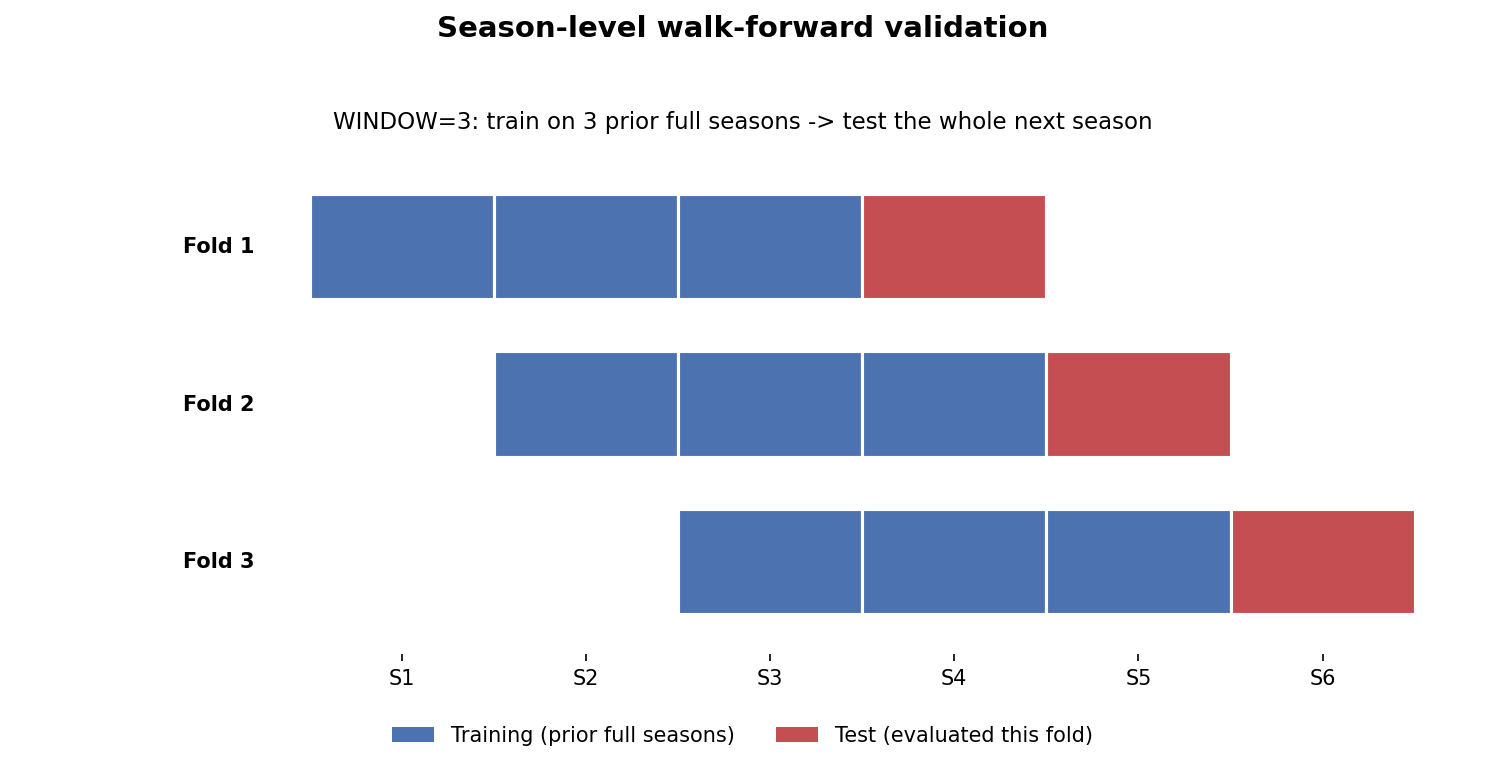
\includegraphics[width=0.7\linewidth]{images/walkforward_scheme.png}
    \caption{Walk-forward scheme }
    \label{fig:walkforward_scheme}
\end{figure}

Walk-forward method is used for two reasons. Firstly, it is necessary to perform some sort of cross-validation in order to reduce randomness and provide robust reliable results that are assumed to be closely replicated if tested on future data. Secondly, as mentioned earlier, reducing the size of training is in this case preferred, as going back in time too far can be counterproductive. The parameter tuning, in this case the parameter being the window size of the walk-forward validation, has revealed that the ideal train set would include 3-4 seasons. On top of the walk-forward validation algorithm, the training consists of within-season chunks that include the freshest set of matches for making predictions as shown in figure \ref{fig:walkforward_intraseason_scheme}.


\begin{figure}[H]
    \centering
    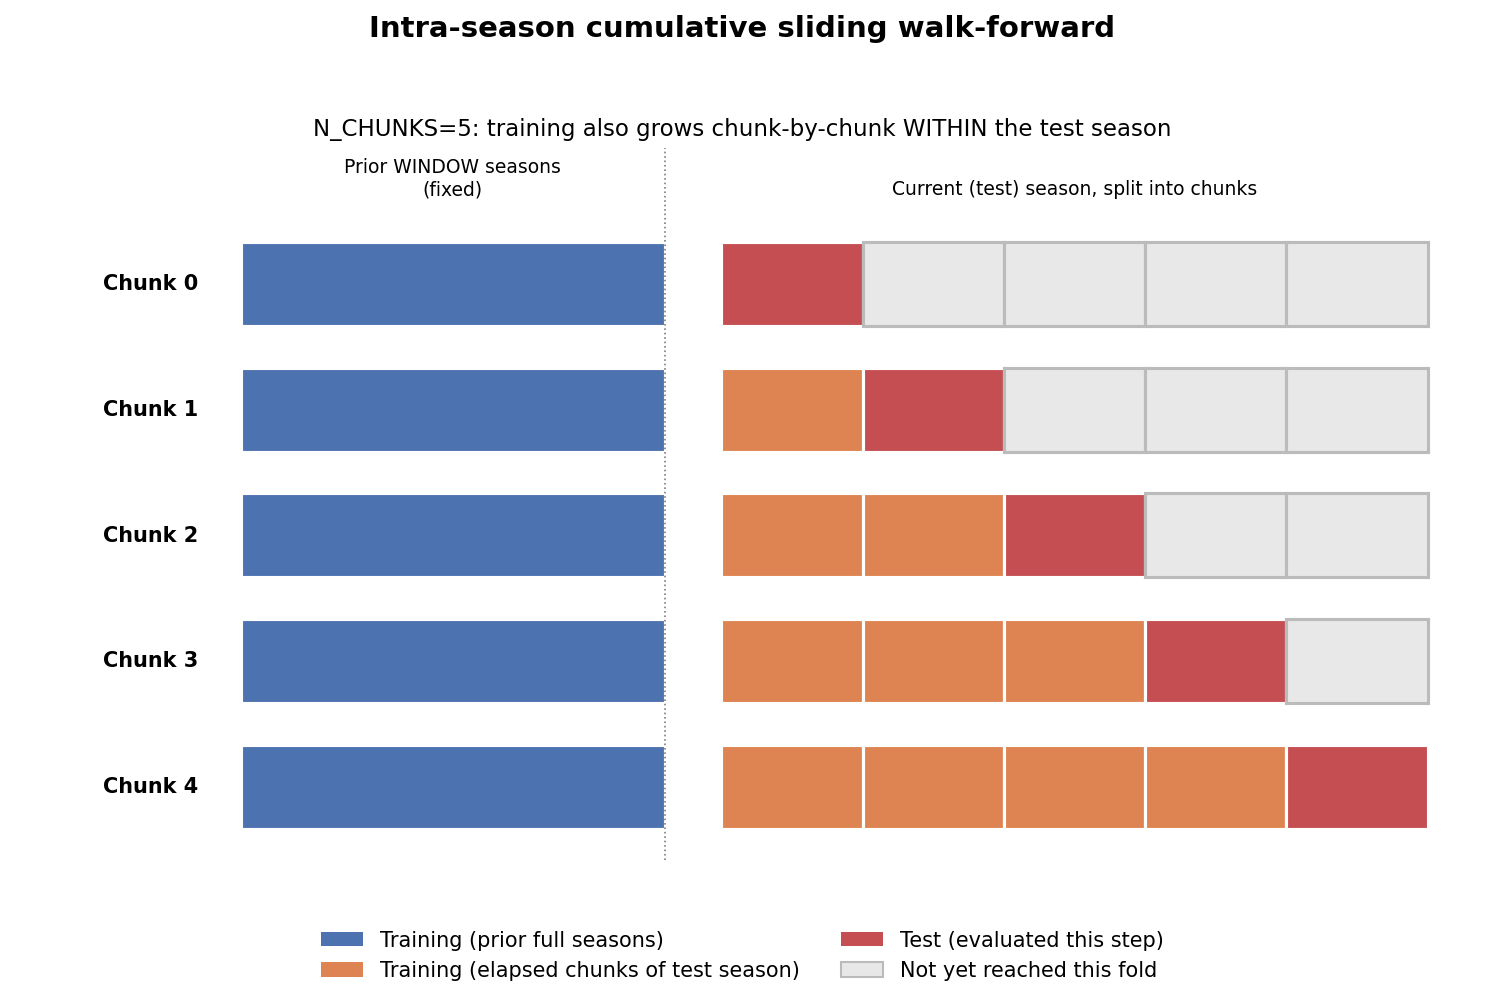
\includegraphics[width=0.7\linewidth]{images/walkforward_intraseason_scheme.png}
    \caption{Walk-forward intraseason scheme }
    \label{fig:walkforward_intraseason_scheme}
\end{figure}

The chunks accumulate over time and for each window of the span of 3 seasons. This means that for each window size, e.g iteration of the walk-forward mechanism, there are actually 5 iterations for each window. There are 9 windows, since there are 12 seasons in total. That also means that the first three seasons from 2014-2016/17 are excluded from testing. In total, there are 9 windows multiplied by 5 cumulative chunks for each, making it 45 iterations of the model. No separate third partition is carved out beyond train/test at this stage because hyperparameter tuning and overfitting checks already happened earlier, per-model where it was necessary, using their own held-out validation folds, which is documented in the following subsections for each model separately.  

\section{Models}
As the title of this paper is hinting at, the goal is to see which machine learning models do well in the task of predicting a football match result. There is a variety of ML models that work on a large spectrum of methods that ultimately aim at the same goal - precise predictions. That is why it might be interesting to look at whether there are any major differences in terms of which some algorithms might be favoured for this particular prediction problem rather than others. Before getting into models' specifics, it is worth mentioning again the shape and size of the training data. Football matches records are in tabular form that contain roughly ~1000 entries per training window that would primarily contain the information from previous matches of each team and numbers (elo, points per game) that describes team's strength. This data is also time-sensitive, meaning that not following the continuity of matches in time would result in invalid machine learning practices.




\subsection{Neural network}
First method on the list is a regular feed-forward neural network, utilizing the \texttt{neural-network} family from \texttt{sklearn}. This is a simple implementation that the package offers and the configurations were set after hyperparameter tuning as follows in listing \ref{lst:mlp_config}.

\begin{lstlisting}[style=pythonstyle, caption={FFNN configuration}, label={lst:mlp_config}]
nn = MLPClassifier(
    hidden_layer_sizes=(8,8),
    activation="relu",
    solver="adam",
    alpha=5.55,
    learning_rate_init=0.001,
    random_state=42
)
\end{lstlisting}
Before the training, data is first scaled by \texttt{sklearn}'s \texttt{StandardScaler} class that centers the data around its mean and scales it based on the variance with the formula 
\begin{equation}
z = \frac{x - \mu}{\sigma}
\end{equation}.

\subsubsection{1-SE rule}
The "1-SE (standard error) rule" was introduced for the neural network as well as some other models in the next subsections. It is a method of finding the best configuration of a model with minimal loss and then selecting hyperparameters such that simplify the model as much as possible to avoid overfitting while still staying within the 1-SE margin from the best performing configuration \cite{HastieTibshiraniFriedman2009ESL}. This process effectively does both hyperparameter tuning and validation folds at the same time. This was an addition to the simplified (for computation purposes) walk-forward CV, where a separate chunk was carved out as a validation set. 
\\
The fine-tuning was ran on two hyperparameters. 
First of them, the hidden layers. Because the data that the model is being fed is of small size relative to the neural nets standard, the selection of the hidden layers that were chosen for fine-tuning was also chosen as for a small model. \texttt{[(8,), (16,), (32,), (8, 8), (16, 8)]}. 
The second variable that went through the fine-tuning sweep was the ridge regression (L2) regularization term referred to as "alpha" in the \texttt{sklearn} implementation. It penalizes the sum of squared coefficients and shrinks the weights close to zero. The default value of alpha that this package uses is 0.0001, so the 5.55 value that is actually used is 55 500 times bigger. This points at the fact that the dataset is substantially smaller than what would typically be used for neural networks. Therefore, the data which already includes high variance must be strongly regularized and the fine-tuning discovered the unusually large L2 term. Using a smaller would result in the model seeing and memorizing patterns in noise.
\\
The selection of both hyperparameters was conducted in accordance with the 1-SE rule.



\subsection{Logistic regression}
A classic machine learning method that models the log-odds based on a linear combination of features. Then uses the softmax function to compute the probabilities of either of the three events (H/D/A) happening. For logistic regression it is also a standard procedure to standardize the data similarly as in neural networks, before training the model. After scaling the features, the configuration of the predictor was as such:

\begin{lstlisting}[style=pythonstyle, caption={Logistic regression configuration}, label={lst:lr_config}]
LR_PARAMS = {"C": 0.001, "penalty": "l2"}
lr = LogisticRegression(max_iter=2000, solver="saga", random_state=42, **LR_PARAMS)

\end{lstlisting}
A minor fine-tuning sweep was conducted via the 1-SE rule on the logistic regression as well, choosing the regularization factor L2 over L1 and the "C" which in this case is also a regularization factor, similar as to the one in FFNN, except that the smaller it is the more regularization, thus higher the penalty term. The variable \texttt{C} just describes the inverse of the strength of the penalty term, be it L1 or L2. The intuition follows the same pattern as in the previous model, and that is the high per-match variance in football requires large regularization terms as to prevent learning on noise and therefore overfitting. 



\subsection{Poisson regression}
Unlike the rest of the discriminative models in this paper, the Poisson regression is a generative one. It is a statistical technique used to model and analyze count data, where the outcome variable represents the number of times an event occurs in a fixed interval of time, space, or any other dimension. It is most appropriate when the values of the response variable are non-negative whole numbers \cite{Poisson_regression}. The key assumption is that the counts follow a Poisson distribution. It has been proven in the EDA section of this paper that the goals scored per match do indeed follow this distribution. That is why Poisson regression can be used in this scenario, specifically to model the number of goals for each team, therefore determining the final match outcome as well. 
\\
The dataset consisting of 96 features mentioned in earlier section of this paper is not being fully trained on in these generative models, as the whole idea behind these methods is to model the goals scored that were found to follow the Poisson distribution, hence training Poisson regression models. Therefore, due to small amount of parameters these models have in the first place as well as consistent results on test sets across the walk forward CV, the Poisson regression models were left out of the overfitting check and deemed unnecessary.

\subsubsection{Dixon-Coles (1997) Poisson goal model}

Each team gets an attack strength and a defense weakness ratio. Both home and away goals are modeled as two Poisson-distributed counts. Home advantage gets also factored in as another ratio term. The assumption about the double Poisson model is that these two distributions are independent, except for one case. A correlation correction $\rho$ is added to address the issue of independent Poisson underestimating the amount of low-scoring matches that actually occur where there are 0-2 goals in total, therefore 4 of the plenty of possible outcomes (0-0, 0-1, 1-0, 1-1). Dixon and Coles motivate this dependence tactically: in a tight, low-scoring game both sides have an incentive to shift toward more cautious, risk-averse play in order to protect the current scoreline, which suppresses further goals for \textit{both} teams simultaneously - a joint effect that two independent Poisson variables cannot represent, and one that fades once the game is no longer close \cite{DixonColes}. This model also introduced the exponential time-weighting decay, which is essentially the same mechanism that is used in the exponential moving weighted average in the feature set. However, this model only ever consumes HomeTeam/AwayTeam/FTHG/FTAG features - team names and their goal counts. 
\\
Parameters that are needed for making a prediction, $\alpha$ - attack strength, $\beta$ - defense strength and $\gamma$ - home advantage are estimated via Maximum likelihood estimation, as there is no closed formula solution. The optimizer chosen was the \texttt{L-BFGS-B} algorithm from \texttt{scipy.optimize.minimize} package, well suited for differentiable functions without constraints. The likelihood function for the Dixon-Coles model is defined as follows: 

\begin{equation}
\mathcal{L}(\boldsymbol{\alpha}, \boldsymbol{\beta}, \gamma, \rho) = \prod_{k=1}^{N} \tau_\rho(x_k, y_k) \cdot \frac{e^{-\lambda_k}\lambda_k^{x_k}}{x_k!} \cdot \frac{e^{-\mu_k}\mu_k^{y_k}}{y_k!}
\end{equation}

\begin{description}
    \item[$N$] Total number of matches in the dataset.
    \item[$x_k$] Actual number of goals scored by the home team in match $k$.
    \item[$y_k$] Actual number of goals scored by the away team in match $k$.
    \item[$\lambda_k$] Expected home goals in match $k$, as defined by $\log(\lambda_k) = \alpha_{i(k)} + \beta_{j(k)} + \gamma$.
    \item[$\mu_k$] Expected away goals in match $k$, as defined by $\log(\mu_k) = \alpha_{j(k)} + \beta_{i(k)}$.
    \item[$\tau_{\rho}(x,y)$] Correction factor applied to the independent Poisson probability for scoreline $(x,y)$. This is what separates the Dixon-Coles model from just a plain double Poisson regression.
    \item[$\rho$] Dependence parameter, estimated jointly with $\alpha$, $\beta$, $\gamma$ via MLE, typically found to be small and negative (around $-0.1$ to $-0.2$ in most fitted football datasets).
\end{description}

The correction factor $\tau$ is defined as follows:
\begin{equation}
\tau_{\rho}(x, y) =
\begin{cases}
1 - \lambda\mu\rho & \text{if } x=0, y=0 \\
1 + \lambda\rho & \text{if } x=0, y=1 \\
1 + \mu\rho & \text{if } x=1, y=0 \\
1 - \rho & \text{if } x=1, y=1 \\
1 & \text{otherwise}
\end{cases}
\end{equation}


A team with no history in the training window (e.g.\ newly promoted) falls
back to average league strength, $\alpha_i = \beta_i = 0$.
\\
After estimating the coefficients on the particular training set, coefficients like shown on an example here are ready for the next stage. The higher the attacking coefficient, the more likely is a team to score more goals, while the lower the defense, the harder it should be for the opposition to score.

\begin{table}[H]
\centering
\begin{tabular}{@{} l c c @{}}
\toprule
\textbf{Team} & \textbf{Attack} & \textbf{Defense} \\
\midrule
Arsenal      & 1.034 & -0.939 \\
Aston Villa  & 0.843 & -0.689 \\
Bournemouth  & 0.812 & -0.652 \\
Brighton     & 0.751 & -0.832 \\
Burnley      & 0.874 & -0.917 \\
Chelsea      & 1.241 & -0.870 \\
\bottomrule
\end{tabular}
\caption{Example of team attack and defense strength ratings}
\label{tab:team_ratings}
\end{table}

The prediction formula using the coefficients from previous step:
\begin{equation}
\log(\lambda_{ij}) = \alpha_i + \beta_j + \gamma
\end{equation}

\begin{equation}
\log(\mu_{ji}) = \alpha_j + \beta_i
\end{equation}

\begin{description}
    \item[$\lambda_{ij}$] Expected number of goals scored by the home team $i$ against away team $j$.
    \item[$\mu_{ji}$] Expected number of goals scored by the away team $j$ against home team $i$.
    \item[$\alpha_i$] Attack strength coefficient of team $i$.
    \item[$\beta_j$] Defense strength coefficient of team $j$.
    \item[$\gamma$] Home advantage coefficient.
\end{description}


\subsubsection{Dixon-Coles Poisson model with Covariates}
The plain Dixon-Coles model has some drawbacks, especially with its naive assumptions. Since the method computes static team ratings, they are not being updated match by match on the current form, which is intuitively a very simple and sub-optimal way of handling the problem. The distinction between the classic Dixon-Coles Poisson model described above and the extension of it with covariates lies in how $\lambda$ and $\mu$ (each team's expected goals) get computed. 
\begin{equation}
\log(\lambda) = \text{home\_adv} + \beta_{\text{home}} \cdot [\text{covariates}]
\end{equation}

\begin{equation}
\log(\mu) = \beta_{\text{away}} \cdot [\text{covariates}]
\end{equation}
Perhaps contrary to intuition, adding more features in this model, unlike only using team name and team goals features in the first model actually produces less parameters. The parameters are shrunk from 2(home and away team)*20(number of teams) + (home advantage + $\rho$) = 42 total to 16 (home advantage + $\beta$ + 2*7(covariates for home and away team)). Team identity is never used directly here; the model only ever sees each team's current features without explicitly assigning a team name to it. The model is working with richer information and fewer parameters, which is a "win-win" situation.
\\
All the 16 parameters are estimated via Maximum likelihood estimation. The log-likelihood function is the same as in the simple Dixon-Coles model, except that $\lambda$ and $\mu$ are computed differently. The initialization of the parameters is as follows: $\beta$ = 0, home\_adv = 0.2, $\rho$ = 0. The covariates variable in the equations represents a vector of features that are used to predict the expected goals for each team. The coefficients $\beta_{\text{home}}$ and $\beta_{\text{away}}$ are estimated for these covariates, allowing the model to capture the influence of various factors on the expected goals scored by each team. The covariates undergo standarization before the optimization takes place, as the coefficients are estimated on a standardized scale. Covariates were selected carefully after running a feature importance analysis in the earlier section of this paper. The final set of covariates that yielded best results were:
\begin{lstlisting}[style=pythonstyle, caption={Selected covariates for the Dixon-Coles covariate model}, label={lst:dc_covariates}]
HOME_COVARIATES = [
    "Home_Elo", "Away_Elo", "Home_xG_Rolling5", "Away_xGA_Rolling5", "Home_PPG",
    "Home_ShotOnTargetDifference_RollingTeam7", "Away_ShotOnTargetDifference_RollingTeam7",
]
AWAY_COVARIATES = [
    "Away_Elo", "Home_Elo", "Away_xG_Rolling5", "Home_xGA_Rolling5", "Away_PPG",
    "Away_ShotOnTargetDifference_RollingTeam7", "Home_ShotOnTargetDifference_RollingTeam7",
]
\end{lstlisting}


\subsubsection{Bivariate Poisson model with Covariates}
\label{sec:bivariate-poisson}
As an extension to the Dixon-Coles model, the bivariate Poisson model with covariates allows for modeling the joint distribution of two count variables (e.g., goals scored by home and away teams) while incorporating covariates. This model captures the potential correlation between the two count variables, which is particularly relevant in football matches where the performance of one team can influence the performance of the other. This is the exact opposite assumption of the key assumption in the Dixon-Coles model, where the two Poisson distributions are assumed to be independent, except for the low-scoring matches. The bivariate Poisson model with covariates allows for a more flexible representation of the relationship between the two count variables, enabling a better and far more realistic understanding of how various factors impact the expected goals for each team \cite{KarlisNtzoufras2003}. This method is therefore a more general approach to modeling football match outcomes as opposed to a hand-patch fix for the dealing with dependence between two variables in low-scoring matches addressed in the Dixon-Coles model. 
\\
Instead of two independent Poisson counts, define three independent Poisson variables $X_1, X_2, X_3$ and set: $$\text{Home} = X_1 + X_3, \qquad \text{Away} = X_2 + X_3$$ $X_3$ is a goals component shared by both teams (interpretable as game pace/tempo), which induces $\mathrm{Cov}(\text{Home}, \text{Away}) = \lambda_3$. $\log\lambda_1$ (home rate, previously denoted as $\lambda$) and $\log\lambda_2$ (away rate, previously denoted as $\mu$) are driven by the exact same 7 standardized covariates as your independent-covariate model. $\lambda_3 = e^\theta$ is a single global scalar that takes over the role of $\rho$ as the model's one correlation parameter. The parameter count remains unchanged at 16 ($\beta_{\text{home}}$ (7) + $\beta_{\text{away}}$ (7) + home\_adv + $\theta$), all still fit jointly via the same L-BFGS-B MLE as before.

\begin{equation}
\mathcal{L}(\boldsymbol{\beta}_{\text{home}}, \boldsymbol{\beta}_{\text{away}}, \gamma, \theta) = \prod_{k=1}^{N} e^{-(\lambda_{1,k}+\lambda_{2,k}+\lambda_3)} \frac{\lambda_{1,k}^{x_k}}{x_k!} \frac{\lambda_{2,k}^{y_k}}{y_k!} \sum_{i=0}^{\min(x_k,y_k)} \binom{x_k}{i}\binom{y_k}{i}\, i! \left(\frac{\lambda_3}{\lambda_{1,k}\lambda_{2,k}}\right)^{i}
\end{equation}
with
\begin{equation}
\lambda_{1,k} = \exp\!\big(\gamma + \mathbf{c}_{\text{home},k} \cdot \boldsymbol{\beta}_{\text{home}}\big), \qquad \lambda_{2,k} = \exp\!\big(\mathbf{c}_{\text{away},k} \cdot \boldsymbol{\beta}_{\text{away}}\big), \qquad \lambda_3 = e^{\theta}
\end{equation}


\begin{description}
    \item[$N$] Total number of matches in the dataset.
    \item[$x_k$] Actual number of goals scored by the home team in match $k$.
    \item[$y_k$] Actual number of goals scored by the away team in match $k$.
    \item[$\mathbf{c}_{\text{home},k}, \mathbf{c}_{\text{away},k}$] Standardized covariate vectors for match $k$ (Elo, rolling xG/xGA, PPG, shot-on-target difference).
    \item[$\lambda_{1,k}, \lambda_{2,k}$] Match-specific home/away scoring rates, driven by the covariates as in the independent covariate model.
    \item[$\lambda_3$] Shared goals component (interpretable as game pace/tempo) inducing $\mathrm{Cov}(X,Y) = \lambda_3$ across every scoreline. Replaces $\rho$ from the Dixon-Coles $\tau$ correction.
    \item[$\theta$] Free parameter estimated jointly with $\boldsymbol{\beta}_{\text{home}}, \boldsymbol{\beta}_{\text{away}}, \gamma$ via MLE, with $\lambda_3 = e^{\theta}$ enforcing $\lambda_3 > 0$ (only non-negative correlation is representable by this construction).
\end{description}

The final prediction of the match outcome is based on:
$$
P(\text{H}) = \sum_{x=1}^{K}\sum_{y=0}^{x-1} P(X{=}x,Y{=}y), \qquad
P(\text{D}) = \sum_{x=0}^{K} P(X{=}x,Y{=}x), \qquad
P(\text{A}) = \sum_{y=1}^{K}\sum_{x=0}^{y-1} P(X{=}x,Y{=}y)
$$
where $K$ is the goal-truncation cutoff (max set to 10 in the code) and the grid ${P(X{=}x,Y{=}y)}_{x,y=0}^{K}$ is renormalized to sum to 1 before these three sums are taken.

\begin{figure}[H]
    \centering
    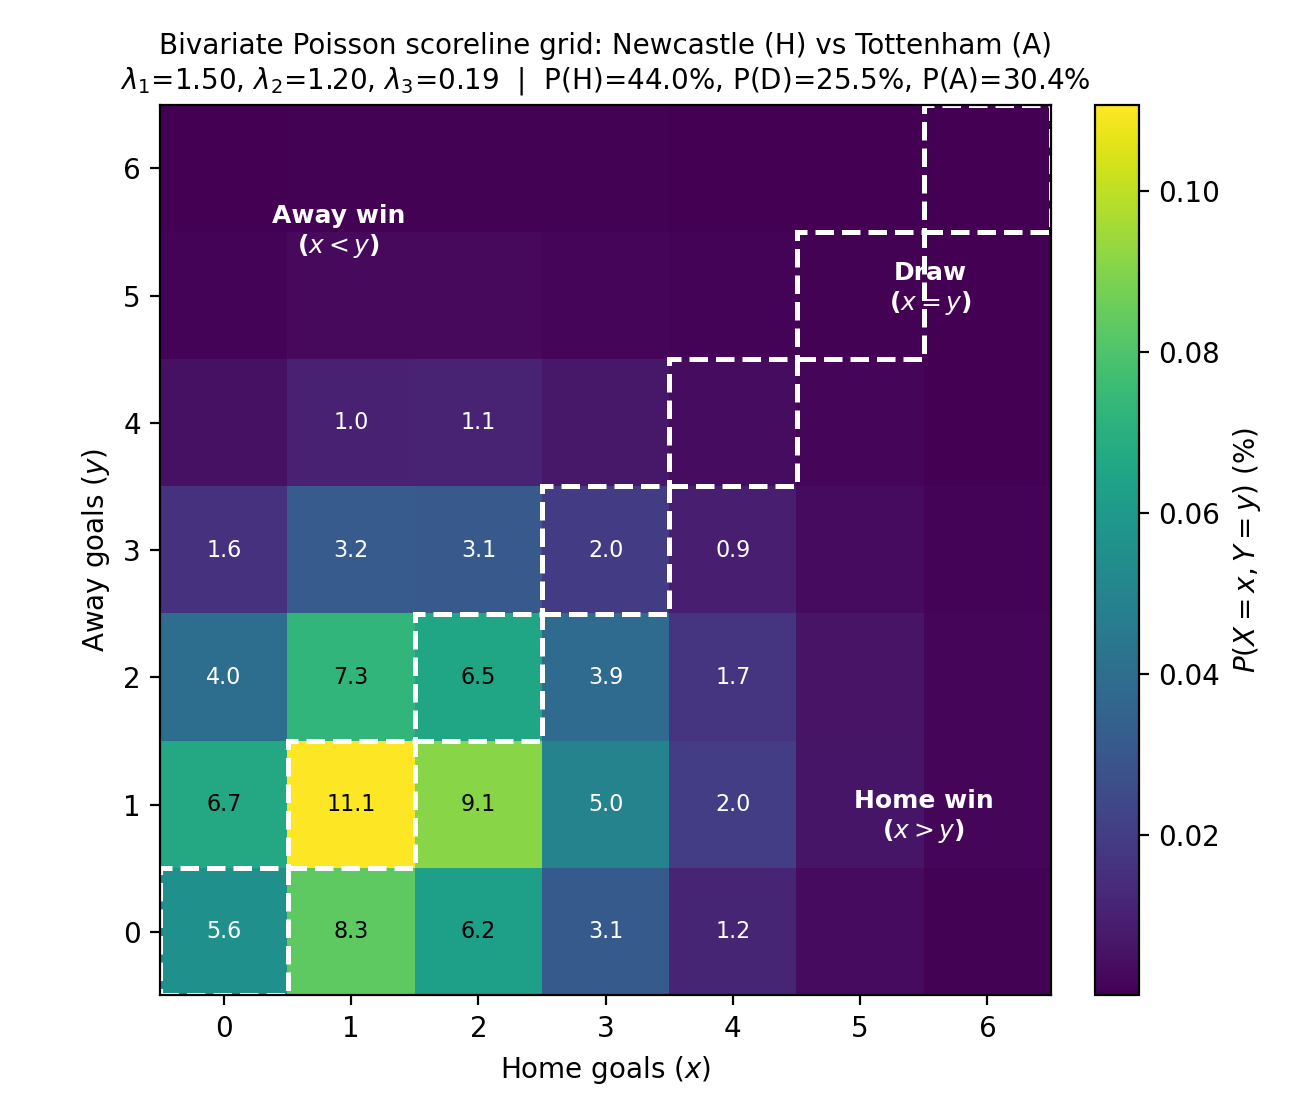
\includegraphics[width=0.75\linewidth]{images/bivariate_grid_example.png}
    \caption{Example scoreline grid $P(X{=}x,Y{=}y)$ from the fitted bivariate Poisson model, for one real match (Newcastle vs.\ Tottenham, 2024-25 season, $K=6$). The dashed cells mark the draw diagonal; summing the grid below/on/above it gives $P(\text{H})$, $P(\text{D})$, $P(\text{A})$ respectively.}
    \label{fig:bivariate_grid}
\end{figure}




\subsection{Ensemble methods}
Machine learning ensembles are a powerful machine learning method utilizing the wisdom of the crowd. The idea is to combine multiple models to produce a more accurate and robust prediction. Two of the popular methods are bagging and boosting. The main representatives of each are Random Forest \cite{Breiman2001RandomForests} and XGBoost \cite{ChenGuestrin2016XGBoost}, respectively, tree based methods that are widely used in many machine learning tasks. These methods are particularly useful in tabular data which happens to be the format of the dataset in this paper. The ensemble methods are also known for their ability to handle high-dimensional data and capture complex relationships between features, making them suitable for the task of predicting football match outcomes.
\subsubsection{Random forest}
Firstly, the bagging ensemble method. It was used throughout the whole project as a reference model, mainly in the feature selection section, where it served as feature importance determiner both in gini impurity based importance as well as permutation score. The same logic for hyperparameter tuning combined with overfitting detection was applied as the other discriminative models in this paper, done via the 1-SE rule. The tuning selection was done on these hyperparameters in listing \ref{lst:rf_finetune}.

\begin{lstlisting}[style=pythonstyle, caption={Selection of RF parameters to be fine-tuned}, label={lst:rf_finetune}]
N_ITER = 60  
    PARAM_DIST = {
    "n_estimators": [100, 200, 300, 500],
    "max_depth": [3, 4, 5, 6, 8, 10],
    "min_samples_leaf": [1, 2, 5, 10, 20, 30],
    "min_samples_split": [2, 5, 10, 20],
    "max_features": ["sqrt", "log2", None],
}
\end{lstlisting}
Due to lack of computation power, \texttt{sklearn}'s \texttt{RandomizedSearchCV} with 60 iterations was the preferred option as opposed to an exhaustive search over all the possible combinations. The following parameters in the listing \ref{lst:rf_params} were then used in the inference after running the simplified walk forward CV with the 60 random iterations.

\begin{lstlisting}[style=pythonstyle, caption={Fine-tuned RF parameters}, label={lst:rf_params}]
rf = RandomForestClassifier(
                n_estimators=200,
                max_depth=4,
                min_samples_leaf=10,
                min_samples_split=5,
                random_state=42,
                n_jobs=-1
            )
proba = rf.predict_proba(X_test)
\end{lstlisting}
The classifier was trained and following that, the output of predicted probabilities for either outcome of a match in order to compute the decimal odds and evaluate.



\subsubsection{XGBoost}
Similarly to random forest, XGBoost is also prone to overfitting and prefers large tabular data. The 1-SE rule that was already mentioned multiple times was also crucial in the case of this gradient boosting method. The same structure of fine-tuning and validating processes as in random forest were applied here as well, except of course different hyperparameters were to be fine-tuned as shown in the listing \ref{lst:xgb_finetune}.

\begin{lstlisting}[style=pythonstyle, caption={Selection of XGB parameters to be fine-tuned}, label={lst:xgb_finetune}]
PARAM_DIST = {
    "n_estimators": [100, 200, 300, 500],
    "max_depth": [2, 3, 4, 5, 6],
    "learning_rate": loguniform(1e-2, 3e-1),
    "subsample": uniform(0.6, 0.4),          # 0.6 - 1.0
    "colsample_bytree": uniform(0.6, 0.4),   # 0.6 - 1.0
    "min_child_weight": [1, 3, 5, 10, 20],
    "reg_alpha": loguniform(1e-3, 1e1),
    "reg_lambda": loguniform(1e-3, 1e1),
}
\end{lstlisting}
The number of iterations of the \texttt{RandomizedSearchCV} was increased to 80 due to the amount of parameters to be swept through.

\newpage
\begin{lstlisting}[style=pythonstyle, caption={Fine-tuned XGB parameters}, label={lst:xgb_params}]
xgb = XGBClassifier(
                n_estimators=200,
                max_depth=4,
                learning_rate=0.05,
                subsample=0.8,
                colsample_bytree=0.8,
                min_child_weight=10,
                random_state=42,
                n_jobs=-1,
                eval_metric="mlogloss",
                early_stopping_rounds=20,
            )

proba = xgb.predict_proba(X_test)
\end{lstlisting}

The parameters such as \texttt{max\_depth} in the listing \ref{lst:xgb_params} indicate that both ensemble methods require shallow trees to prevent overfitting on the dataset used. On top of that, the XGBoost has an early stopping mechanism that prevents it from learning too many patterns which at some point carry more of noise than genuine signal.  




\subsection{SVM}
SVMs are a machine learning method that finds the maximum-margin separating hyperplane between classes; via the kernel trick, this boundary can also be implicitly non-linear in the original feature space without ever computing the transformed features directly. They generally work well with small-mid sized data and that is why they are also part of the experiment. Standardization of the data before training SVMs is a very important preprocessing step since distances play huge role in determining the hyperplane.
\subsubsection{Simple SVM}
As the EDA showed earlier, there are patterns that occur in the data that are not of linear shape, so the kernel of choice in the SVM is the radial one. The 1-SE rule for overfitting detection and fine-tuning was once again applied. The terms that were fine-tuned were C and $\gamma$. A smaller C widens the margin of the decision boundary, allowing more misclassified training points in exchange for less overfitting. The other factor, $\gamma$, is specifically part of the radial kernel. It regularizes each point's influence, which is again closely tied to the overfitting issue.

\subsubsection{SVM with UMAP}
As part of this experiment, another kind of setup is introduced in the last subsection of the machine learning methods of this paper. A new method that combines dimensionality reduction with a predictive model. First, the UMAP dimensionality reduction takes place, which unlike e.g PCA does not assume linearity.  It is an unsupervised method and it preserves neighborhood structure in feature space, with no notion of what's predictive of match outcome \cite{McInnesHealyMelville2018UMAP}. The idea behind this method is to reduce feature space which the SVM could potentially benefit from. The one parameter here that was fine-tuned was \texttt{n\_components}, the number of dimensions UMAP reduces the original feature space down to. Figure~\ref{fig:umap_ncomponents} shows the sweep: validation log loss stays essentially flat across the tested range (a spread of only about 0.002), so \texttt{n\_components} has little effect on performance here rather than a clear, sharply-defined optimum. The final model uses \texttt{n\_components}=15, which sits within this flat region and performs on par with the sweep's nominal minimum.


\begin{figure}[H]
    \centering
    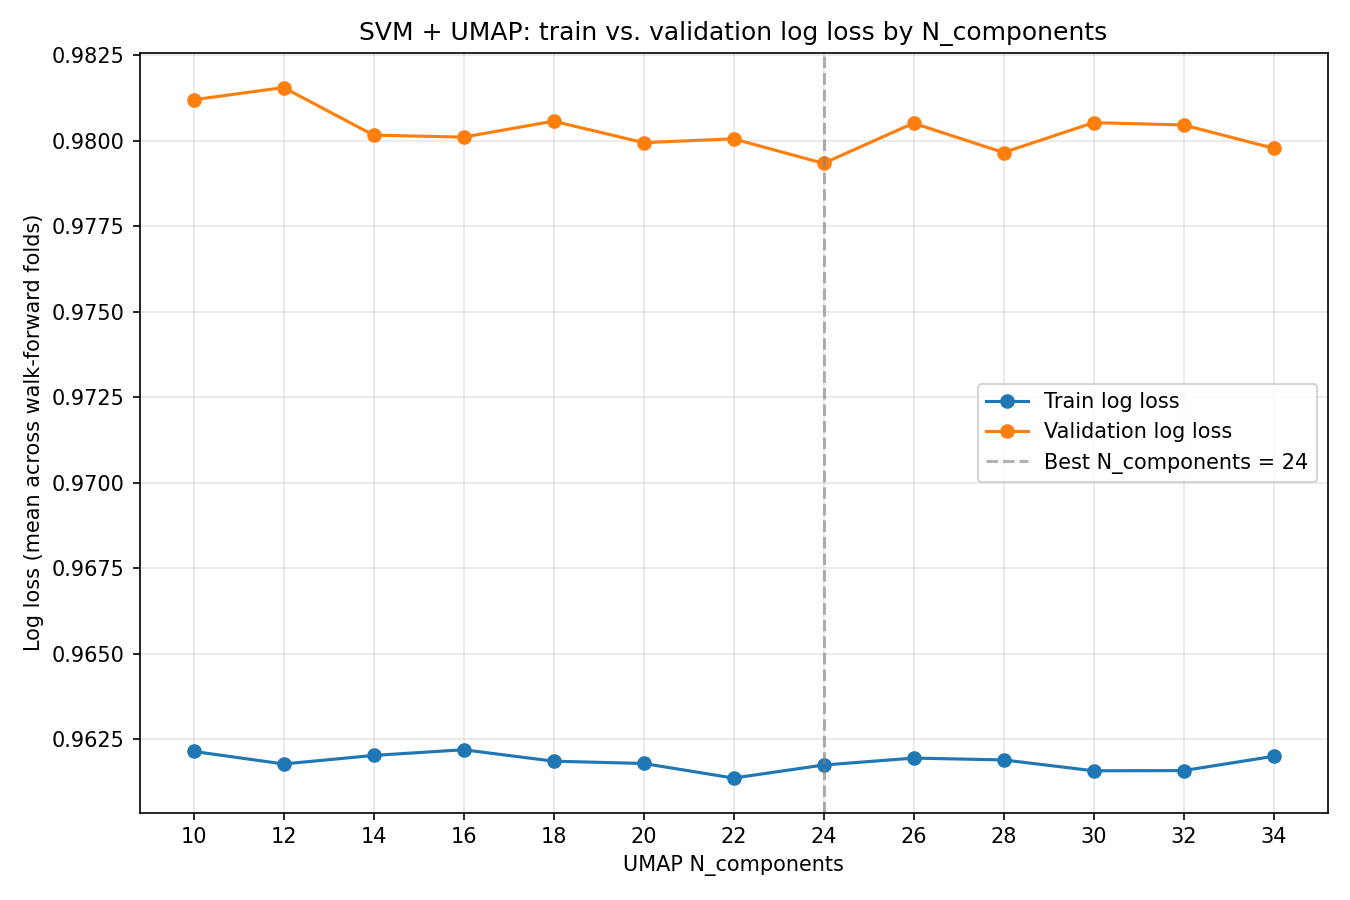
\includegraphics[width=0.75\linewidth]{images/umap_ncomponents_sweep.png}
    \caption{The sweep to find the optimal number of \texttt{n\_components} in the UMAP dimensionality reduction method.}
    \label{fig:umap_ncomponents}
\end{figure}


\section{Evaluation methods}
The ultimate goal of the models in 1X2 betting is to produce probabilistic output. In this paper, predictions are firstly treated as a classification problem. The model simply predicts the outcome of a match. This is already a great and interpretable way in order to carry out feature engineering, which is pivotal to increasing the accuracy and F1 score. However, accuracy, defined as the proportion of correctly predicted outcomes, is widely used but insufficient for probabilistic outputs\cite{MLeval}. This is due to the need for a way to measure the quality of probabilistic predictions. The accuracy would not capture the uncertainty in the model's predictions, and that is the very essential task in the odds production. What is a much more insightful metric for evaluating probabilistic predictions is the logarithmic loss (log loss), which measures the performance of a classification model where the prediction input is a probability value between 0 and 1. Log loss increases as the predicted probability diverges from the actual label. A perfect model would have a log loss of 0. The log loss is defined as follows:
$$\text{LogLoss} = -\frac{1}{N} \sum_{t=1}^{N} \sum_{i=1}^{R} o_{ti} \log(f_{ti})$$

Equivalently, since $o_{ti}=1$ only for the realized outcome and 0 otherwise, this collapses to just the log-probability the model assigned to what actually happened:

$$\text{LogLoss} = -\frac{1}{N} \sum_{t=1}^{N} \log(f_{t, y_t})$$
Another way of measuring the quality of probabilistic predictions is the Brier score. It is a strictly proper scoring rule that measures the accuracy of probabilistic predictions. The Brier score, similarly to log loss, is applicable to tasks in which predictions must assign probabilities to a set of mutually exclusive discrete outcomes or classes. \cite{wiki:Brier}. 

The multi-category (multinomial) Brier Score generalizes the binary case to a set of mutually exclusive discrete outcomes or classes \cite{wiki:Brier}.

\begin{equation}
BS = \frac{1}{N} \sum_{t=1}^{N} \sum_{i=1}^{R} \left( f_{ti} - o_{ti} \right)^2
\end{equation}

\begin{description}
    \item[$N$] Total number of forecast instances (e.g., matches).
    \item[$R$] Total number of mutually exclusive outcome categories (e.g., $R=3$ for home win, draw, away win).
    \item[$f_{ti}$] Forecast probability assigned to category $i$ for instance $t$, where $\sum_{i=1}^{R} f_{ti} = 1$.
    \item[$o_{ti}$] Binary indicator for the actual outcome: $o_{ti} = 1$ if category $i$ occurred for instance $t$, and $o_{ti} = 0$ otherwise.
\end{description}

It is therefore a much preferred method to evaluating probabilistic outcomes than accuracy, which disregards the magnitude of hits and misses completely. The Bries loss evaluation method comes at a cost of low interpretability, compared to raw accuracy. However, first introduced in weather forecast, the Brier skill score can handle this as well. The Brier Skill Score (BSS) expresses the relative improvement of a forecast model over a reference forecast, such as climatology (long-run base rates) or a naive baseline \cite{BSS}.

\begin{equation}
BSS = 1 - \frac{BS_{\text{forecast}}}{BS_{\text{reference}}}
\end{equation}

\begin{description}
    \item[$BS_{\text{forecast}}$] Brier Score of the model being evaluated.
    \item[$BS_{\text{reference}}$] Brier Score of the reference (baseline) forecast.
    \item[$BSS$]Skill score, where $BSS > 0$ indicates the forecast model outperforms the reference, $BSS = 0$ indicates no improvement, and $BSS < 0$ indicates the model performs worse than the reference.
\\
\\
In the case of this paper, the reference that is being compared to the models' predictions is a concept called climatological probability. First introduced in 1950\cite{Climatology}, it works on the same principle as a naive model that guesses randomly, except that it has knowledge of the real distribution of classes (H/D/A). After computing the BSS of both the models and the market odds, comparison can be made between these two scores. 
\end{description}


\section{Results and discussion}

Log loss and the Brier score (BS) metrics are averaged across the 45 iterations (3236 out-of-sample predictions) of the walk-forward validation. As described before, this method works purely as a final stage testing mechanism, since it is strictly training a model on a certain window in time and consequently tested on an \textbf{unseen} chunk of data (time-wise right after the training window), preventing data leakage. It is implemented as a more robust and insightful way of evaulating the performance of models. 
\\
The accuracy is computed as the total number of correct \texttt{argmax} predictions divided by the total number of matches in the test set. The p-value is calculated using a paired t-test comparing the log loss of each model over all the 45 iterations against the log loss of BET365's odds, which serves as a benchmark for comparison. The Brier Skill Score (BSS) is computed relative to the climatological probability baseline, which has been addressed in the evaluation section.


\begin{table}[H]
\centering
\caption{Model evaluation results (intra-season walk-forward validation, pooled over 3236 matches)}
\label{tab:model_results}
\begin{tabular}{lccccc}
\toprule
\textbf{Model} & \textbf{Log Loss} & \textbf{BS} & \textbf{Accuracy} & \textbf{\textit{p}-value vs.\ BET365} & \textbf{BSS} \\
\midrule
Logistic Regression       & 0.9752 & 0.5795 & 53.92\% & 0.000006     & 10.24\% \\
FFNN                       & 1.0002 & 0.5950 & 51.92\% & $<0.000001$  & 7.84\% \\
Random Forest              & 0.9835 & 0.5845 & 52.53\% & $<0.000001$  & 9.47\% \\
XGBoost                    & 0.9923 & 0.5903 & 52.32\% & $<0.000001$  & 8.57\% \\
SVM (all features)         & 1.0028 & 0.5975 & 52.35\% & $<0.000001$  & 7.45\% \\
SVM (UMAP)                 & 0.9889 & 0.5880 & 53.37\% & $<0.000001$  & 8.92\% \\
\midrule
Poisson (Dixon-Coles)              & 0.9845 & 0.5855 & 52.56\% & $<0.000001$ & 9.31\% \\
Poisson (Dixon-Coles + Covariates) & 0.9733 & 0.5780 & 53.74\% & 0.000410    & 10.47\% \\
Poisson (Bivariate)                & 0.9678 & 0.5746 & 54.26\% & 0.030035    & 11.00\% \\
\midrule

\midrule
Market (avg.\ bookmaker)  & 0.9607 & 0.5697 & 54.60\%     & ---          & 11.76\% \\
BET365                     & 0.9615 & 0.5700 & 54.70\% & ---          & 11.71\% \\
\bottomrule
\end{tabular}
\end{table}


The key metrics to evaluating probabilistic models are the log loss and the Brier score even though the accuracy follows the trend of the other two metrics and is reported here for completeness. The table shows the distinction between discriminative and generative models. The discriminative models, which include logistic regression, feed-forward neural networks, random forest, XGBoost, and SVMs, generally perform worse than the generative Poisson models in terms of log loss and Brier score. 


\subsection{Discriminative models}
When fine-tuning the SVM model trained on all 96 features of the dataset, no improvement of performance was detected, on the contrary, the log loss slightly increased despite the overfitting gap between train and validation set shrinking by a significant amount. This indicates that perhaps the feature space is large, the nature of it does not fit the SVM well or the multicollinearity is an issue. To test this hypothesis, UMAP dimensionality reduction was applied to the dataset before testing the SVM again, which showed a significant improvement in performance of the SVM. In any case, the plain SVM trained on all the features was the worst predictor in the whole paper and the UMAP version's improvement was not enough to consider this machine learning method as adequate for football 1X2 predictions. The results show that there are plenty of better models available just in this paper.
\\
The results of predictions made by FFNN could also be labeled as a failure. While deep learning has its strength especially in large scale feature spaces and it greatly benefits from plethora of dat entries, this particular problem is not fit for such type of model. The experiments in this paper were conducted on data from a single league, therefore limited amount of matches. However, adding more leagues would arguably still not produce significantly better results by a neural network as it would only be a few-fold size of increase, not mentioning all the other issues that would bring. To sum up the neural network experiment, it was the second worst on the main metrics of probabilistic outputs and even the worst on the accuracy metric. Threeway football betting is not one of neural networks' strengths.
\\
The ensemble methods were from the beginning expected to perform quite well given the tabular nature of data. Both random forest and xgboost were however sub-optimal choices as it was revealed later by the generative models. These models, similarly to neural networks, benefit largely from the sheer amount of data they are given. This is the same issue addressed earlier -- high-capacity models suffering from small and noisy datasets. On the other hand, logistic regression does not have the same limitation and produced very promising and optimistic results. Despite being on the simpler side of models complexity, it produced the best result out of all discriminative models and the third best result overall in this paper, just fell marginally short of the Dixon-Coles model with covariates. Assumption about the reason for great success of logistic regression is that the objective function of it is directly maximizing likelihood i.e. directly minimizing log loss, which happens to be the exact metric of all models' performances.


\subsection{Poisson regression models}
Among the Poisson models, the bivariate Poisson model with covariates achieves the best performance, indicating that advancing from the naive assumption of independence of goal counts in Dixon-Coles models by introducing a third variable that represents a shared goals component  (interpretable as game pace/tempo) and incorporating relevant covariates leads to more accurate predictions. All the models tested fall short of the market odds, however, some more than others. The bivariate Poisson model's p-value after the paired t-test of log-loss across all 45 iterations is 0.030035, which is below the significance level of 0.05, indicating that its performance is statistically significantly different from BET365's odds on the 95\% confidence interval. However, conducting a t-test with a 99\% confidence interval would not reject the null hypothesis that the log loss of the model and BET365's odds come from a different distribution. This is a strong indication that the model is performing close to the market odds. Moreover, the BSS proves to be stably positive for all models meaning they comfortably beat the climatological probability baseline. The BSS of the bivariate Poisson model is 11.00\%, which is only 0.76\% lower than the market odds, thus providing another proof of the model's stong performance.
As a food for thought, after implementing all the other techniques that bookmakers use in order to maximise their profit that were mentioned in the Bookmaker section, it would very likely lead to the bivariate Poisson model being fully competitive with the market. 



To illustrate what the walk-forward scheme actually produces under the hood, Table~\ref{tab:bivariate_per_season} shows the bivariate Poisson model with covariates (Section~\ref{sec:bivariate-poisson}, the best-performing model in Table~\ref{tab:model_results}) with the same configuration as in all the other results ($\texttt{WINDOW}=3$, $\texttt{N\_CHUNKS}=5$) re-run and broken out by test season, rather than pooled into a single row.

\begin{table}[H]
\centering
\begin{tabular}{llcccc}
\toprule
\textbf{Test season} & \textbf{Source} & \textbf{Matches} & \textbf{Mean log loss} & \textbf{Mean BS} & \textbf{Accuracy} \\
\midrule
\multirow{3}{*}{2017-18} & Model      & \multirow{3}{*}{359} & 0.9438 & 0.5604 & 54.60\% \\
                          & BET365     &                       & 0.9406 & 0.5571 & 55.43\% \\
                          & Avg-bookie &                       & 0.9398 & 0.5565 & 55.43\% \\
\midrule
\multirow{3}{*}{2018-19} & Model      & \multirow{3}{*}{360} & 0.8988 & 0.5274 & \textbf{60.28\%} \\
                          & BET365     &                       & 0.8977 & 0.5255 & 58.33\% \\
                          & Avg-bookie &                       & 0.8983 & 0.5258 & 58.33\% \\
\midrule
\multirow{3}{*}{2019-20} & Model      & \multirow{3}{*}{360} & \textbf{0.9743} & 0.5769 & \textbf{53.33\%} \\
                          & BET365     &                       & 0.9763 & 0.5767 & 52.78\% \\
                          & Avg-bookie &                       & 0.9759 & 0.5768 & 52.78\% \\
\midrule
\multirow{3}{*}{2020-21} & Model      & \multirow{3}{*}{358} & 1.0281 & 0.6120 & 49.16\% \\
                          & BET365     &                       & 1.0121 & 0.6026 & 50.56\% \\
                          & Avg-bookie &                       & 1.0096 & 0.6011 & 50.28\% \\
\midrule
\multirow{3}{*}{2021-22} & Model      & \multirow{3}{*}{360} & 0.9542 & 0.5651 & 55.56\% \\
                          & BET365     &                       & 0.9435 & 0.5584 & 57.50\% \\
                          & Avg-bookie &                       & 0.9425 & 0.5582 & 57.22\% \\
\midrule
\multirow{3}{*}{2022-23} & Model      & \multirow{3}{*}{360} & 0.9708 & 0.5763 & 53.06\% \\
                          & BET365     &                       & 0.9623 & 0.5704 & 56.39\% \\
                          & Avg-bookie &                       & 0.9617 & 0.5704 & 56.67\% \\
\midrule
\multirow{3}{*}{2023-24} & Model      & \multirow{3}{*}{359} & 0.9284 & 0.5474 & \textbf{59.05\%} \\
                          & BET365     &                       & 0.9164 & 0.5384 & 59.33\% \\
                          & Avg-bookie &                       & 0.9168 & 0.5386 & 58.77\% \\
\midrule
\multirow{3}{*}{2024-25} & Model      & \multirow{3}{*}{360} & \textbf{0.9809} & \textbf{0.5857} & 53.33\% \\
                          & BET365     &                       & 0.9822 & 0.5868 & 53.33\% \\
                          & Avg-bookie &                       & 0.9820 & 0.5870 & 53.33\% \\
\midrule
\multirow{3}{*}{2025-26} & Model      & \multirow{3}{*}{360} & 1.0313 & 0.6207 & \textbf{50.00\%} \\
                          & BET365     &                       & 1.0224 & 0.6145 & 48.61\% \\
                          & Avg-bookie &                       & 1.0195 & 0.6132 & 48.61\% \\
\midrule
\multirow{3}{*}{\textbf{Pooled}} & Model      & \multirow{3}{*}{3236} & 0.9678 & 0.5746 & 54.26\% \\
                                  & BET365     &                        & 0.9615 & 0.5700 & 54.70\% \\
                                  & Avg-bookie &                        & 0.9607 & 0.5697 & 54.60\% \\
\bottomrule
\end{tabular}
\caption{Bivariate Poisson model with covariates vs.\ BET365 and average-bookmaker odds (the margin was subtracted so the probabilities sum to 1), intra-season walk-forward broken out by test season. The pooled block matches Table~\ref{tab:model_results}.}
\label{tab:bivariate_per_season}
\end{table}

While the pooled metrics across all seasons are in market's favour, the best performing model in this paper has managed to achieve best season-centric metrics in some cases, highlighted with bold font in Table~\ref{tab:model_results}.
Performance is clearly not stable across seasons: mean log loss ranges from 0.8988 (2018-19) to 1.0313 (2025-26), a gap comparable in size to the difference between the weakest and strongest models. The 2020-21 season (played behind closed doors due to Covid) and the most recent season, 2025-26, are the two worst-performing test seasons, consistent with the home-advantage disruption noted in the EDA section for the former, while the latter is plausibly explained by the model having the least amount of recent within-season data to condition on as well as extraordinarily high amount of draws, effectively making it the hardest season to predict for the models in this paper as well as the market itself. The results from this table are also the practical justification for the walk forward validation method, thus reporting metrics pooled across all 45 walk-forward iterations rather than trusting the result of any single season in isolation.

\begin{figure}[H]
    \centering
    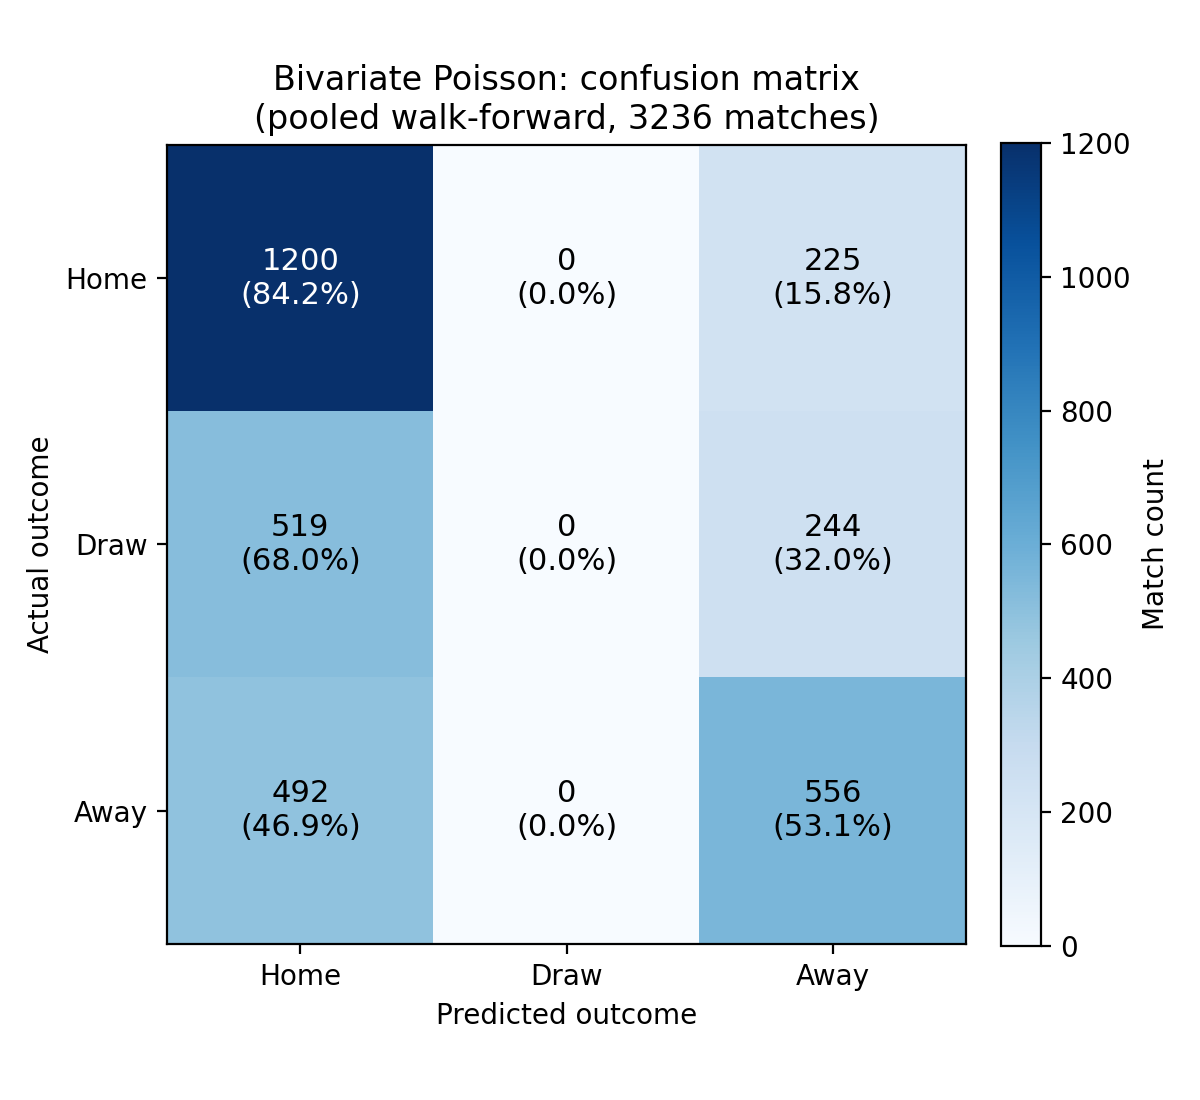
\includegraphics[width=0.7\linewidth]{images/bivariate_confusion_matrix.png}
    \caption{Confusion matrix for the bivariate Poisson model with covariates, pooled across all 45 walk-forward iterations (3236 matches). Percentages are row-normalized (recall per actual outcome).}
    \label{fig:bivariate_confusion}
\end{figure}

Figure~\ref{fig:bivariate_confusion} reveals a limitation that the pooled accuracy figure alone does not: the model never predicts a draw as the single most likely outcome, across all 3236 matches. Of the 763 matches that actually ended in a draw, 519 (68.0\%) were predicted as a home win and 244 (32.0\%) as an away win - not one was predicted as a draw. This is not a bug but a direct consequence of using the single most probable class (argmax) as the prediction: since draws are consistently the least likely of the three outcomes for almost every match (as shown in the EDA section), some other outcome almost always edges them out as the top pick, even when the model assigns a draw a meaningful, non-negligible probability. This is precisely why log loss and the Brier score, which credit the full probability distribution rather than only the top prediction, are the more appropriate metrics for this task, as argued in the Evaluation methods section - accuracy alone would make it look as though the model has no notion of draws at all, which is not the case. Therefore the confusion matrix is shown here just as a qualitative analysis supplementary figure.




\section{Conclusion}
None of the methods tested in this paper were on equal ground with the market odds for prediction of the final outcomes in EPL football matches despite the low disparity in the result metrics (0.0421 difference in log loss between the worst performing model (SVM) and the market). The best performing model was the bivariate Poisson model with covariates, achieving just 0.0071 higher log loss than the market, thus being marginally worse in performance. This is a strong indication that if complemented by techniques outside of pure feature engineering and machine learning that were not part of the objective of this paper, the flagship model in this paper would be competitive with the odds market. Other machine learning methods that were based on discriminative prediction turned out to be less effective, although logistic regression showed promising results. 



\section{Limitations and future research}
As a multi-billion dollar industry, the sports betting market is highly competetive and efficient. These companies have an abundance of resources and data at their disposal, which allows them to create highly accurate odds. 
\\
The models were trained on a dataset of 12 seasons of just a single league. Some machine learning models, such as neural networks or ensemble methods might suffer heavily from the lack of data, therefore also resulting in overfitting which had to be addressed with an unusually large regularization parameter, which is effectively a hand-patch rather than a real solution to the issue. Regarding the SVMs, it is a whole observable structural mismatch between the task and the model. The fact that the fine-tuning process only worsened the performance clearly shows that SVMs are not a good choice for such predictions, especially with a high-dimensional heavily correlated feature space. The logic behind having newly promoted teams in EPL is also not always bullet-proof. For example, in the bivariate Poisson model, the parameters of a new team are hard-coded to a value 0. The Bayesian hierarchical Dixon-Coles \cite{BaioBlangiardo2010BayesianDixonColes}would elegantly fix this issue by shrinking each team's attack/defense strengths toward the league mean proportionally to their number of matches played. Another limitation of the strongest model in the paper was the $\lambda_3$ coefficient which could mathematically only produce non-negative correlation between home and away team goals. A copula-based bivariate goal model \cite{McHaleScarf2011Copula} allows for both positive and negative correlations by coupling two marginal Poisson distributions via Gaussian copula. 
\\
The models tested in this paper were trained only on one sort of data, which is the historical data.This data is naive and in limited size. It is another substantial factor that could hinder the performance. Models trained in this paper were not exposed to any other matches throughout the season than the EPL itself. This means that they cannot recognize that a team might be fatigued because of a challenging match it has played just three days ago across the continent in a different competition. While the historical data used for predictions indeed represents the core of any predictive model for such tasks, novel data including transfers of players, current line-ups, formations, injuries, coach changes, insider information or even weather conditions can all have a tiny impact on the performance by each on their own, however, adding this information on top of the historical data could possibly overcome the small but significant edge that the market has. 
\\
Future research could also be conducted on other machine learning or statistical methods. For example, this is a time-series prediction task but it has not been entirely treated as one. The features are handcrafted as EWMA for a 14 matches window. Models like recurrent neural network (RNN) or long short-term memory (LSTM) neural network could learn their own memory function from data instead of manually choosing it as was done in the paper.
\\
To sum up this section as well as the report itself, there are countless ways to conduct a research on this topic with plethora of different configurations, such as feature set(add-ons to the existing historical data with novel information which could marginally boost up the performance), scale of the data (including more leagues), different machine learning methods such as introduction of new kind of architecture - sequential models or new  algorithmic tweaks like the ones in this section that hint at some improvements of the strongest method in this paper. As already mentioned throughout this paper, including important information about the match that does not only come from historical data would be also an option as well as considering the teams' individual programmes and fixtures that do not only involve the EPL itself, but also other tournaments or even friendly preparation matches that they play. In summary, the results of this paper are therefore not conclusive and should be treated as a starting point for further research in this area.





\printbibliography



\end{document}
